\documentclass[11pt]{article}

\usepackage[margin=1in]{geometry}
\usepackage{amsmath,amssymb,amsthm}
\usepackage{mathtools}
\usepackage{bm}
\usepackage{hyperref}
\usepackage{listings}
\usepackage{xcolor}
\usepackage{booktabs}
\usepackage{enumitem}
\usepackage{tikz}
\usetikzlibrary{shapes.geometric,arrows.meta,positioning,fit}
\usepackage{float}

\newcommand{\dg}{^{\dagger}}
\newcommand{\Neff}{N_{\mathrm{eff}}}
\newcommand{\Nphys}{N_{\mathrm{phys}}}
\newcommand{\Ng}{N_{g}}
\newcommand{\Hqp}{H_{\mathrm{qp}}}
\newcommand{\Himp}{H_{\mathrm{imp}}}
\newcommand{\Hloc}{H_{\mathrm{loc}}}
\newcommand{\trip}[1]{\mathrm{tri}(#1)}

\lstset{
  basicstyle=\ttfamily\small,
  breaklines=true,
  columns=fullflexible,
  frame=single,
  numbers=none,
  language=Python,
  keywordstyle=\color{blue},
  commentstyle=\color{gray}
}

\title{Ghost Gutzwiller Approximation for the Half-Filled Hubbard Dimer:\\
Equations, Conventions, and Numerical Implementation}
\author{gGut\_mau project --- \texttt{gga\_dimer.py}}
\date{\today}

\begin{document}
\maketitle
\tableofcontents

\bigskip
\noindent\textbf{Purpose of this note.} This document is a pedantic, self-contained
description of \emph{exactly} what the code in \texttt{gga\_dimer.py} computes: every
equation, every index convention, every regularization constant, and every numerical
safeguard, together with the reasoning behind each choice. It is meant to let a reader
reproduce the code from the equations alone, or verify the code against the equations
line by line. Physical background (the ghost Gutzwiller approximation, gGA) is kept to
the minimum needed to fix notation; references to the original literature are given in
Section~\ref{sec:refs}.

\section{Physical model}
\label{sec:model}

We study the two-site (``dimer'') single-band Hubbard Hamiltonian
\begin{equation}
  H_{\mathrm{phys}} \;=\; -t\sum_{\sigma=\uparrow,\downarrow}
      \left( c^{\dagger}_{0\sigma} c_{1\sigma} + c^{\dagger}_{1\sigma} c_{0\sigma}\right)
      \;+\; U\sum_{i=0,1} n_{i\uparrow} n_{i\downarrow}
      \;-\; \mu \sum_{i=0,1}\left(n_{i\uparrow}+n_{i\downarrow}\right),
  \label{eq:Hphys}
\end{equation}
with sites labeled $i=0,1$, one physical orbital per site
($\Nphys=1$), and both spins present. The hopping amplitude $t$ sets the energy
unit; the code always uses $t=1$ unless stated otherwise (the CLI flag \texttt{-{}-t}
allows changing it, and every energy reported by the code is implicitly in units
of $t$).

\paragraph{Half filling and particle-hole symmetry.} The chemical potential is
fixed to the particle-hole symmetric value
\begin{equation}
  \mu = U/2 ,
\end{equation}
which pins the total occupation to $\langle n_{0\sigma}+n_{0\bar\sigma}+n_{1\sigma}+n_{1\bar\sigma}\rangle=2$
(one electron per spin, summed over both sites) for \emph{any} $U$. This is the only
filling considered by the code; there is no doping/chemical-potential scan.

\paragraph{Exact benchmark.} \texttt{exact\_dimer.py} diagonalizes
Eq.~\eqref{eq:Hphys} exactly in the full $2^4=16$-dimensional Fock space of the
four physical modes ($i\in\{0,1\}$, $\sigma\in\{\uparrow,\downarrow\}$), by
building the four fermionic annihilation operators via an explicit
Jordan--Wigner string (see Section~\ref{sec:JW} for the general construction,
which is shared with the impurity solver). It reports the ground-state energy
$E_0$, total filling $\langle n\rangle$, and the double occupancy per site
$\mathrm{docc}=\tfrac12\sum_i\langle n_{i\uparrow}n_{i\downarrow}\rangle$, used
throughout as the ground truth that the gGA approximation is checked against.

\section{The ghost Gutzwiller ansatz: general framework}
\label{sec:gga-general}

The ghost Gutzwiller approximation (gGA) approximates the ground state of
Eq.~\eqref{eq:Hphys} variationally as $|\Psi_G\rangle = P|\Psi_{\mathrm{qp}}\rangle$,
where $|\Psi_{\mathrm{qp}}\rangle$ is the Slater-determinant ground state of an
auxiliary, purely quadratic \emph{quasiparticle} Hamiltonian $\Hqp$, and $P$ is a
Gutzwiller-type projector onto the physical Hilbert space. In the standard
(``rotationally invariant slave boson''/gGA) formulation, the projector is
replaced by an equivalent \emph{embedding} (impurity) problem, and the whole
scheme reduces to a self-consistency loop between:
\begin{enumerate}
  \item a one-body quasiparticle Hamiltonian $\Hqp(R,\lambda)$, built from a
    \emph{renormalization matrix} $R$ and an \emph{onsite potential} $\lambda$,
    and
  \item a many-body \emph{impurity} Hamiltonian $\Himp(V,\lambda^c)$, describing
    one physical (correlated) orbital coupled to $\Neff$ auxiliary
    (``ghost'') bath orbitals through a hybridization $V$ and a bath-onsite
    potential $\lambda^c$.
\end{enumerate}

\paragraph{Dimension bookkeeping.} Let $\Nphys$ be the number of physical
orbitals per fragment (here $\Nphys=1$: one site, one orbital, spin handled
symmetrically) and let $\Ng$ be the number of \emph{extra} ghost bath orbitals
requested by the user, on top of the single bath orbital that even the
\emph{non-ghost} (ordinary) Gutzwiller/slave-boson theory already has. Define
\begin{equation}
  \Neff \;=\; \Nphys + \Ng \;=\; 1 + \Ng .
\end{equation}
$\Ng=0$ is \emph{not} ``no bath''; it is the ordinary single-bath Gutzwiller
theory. Each fragment's embedding Hamiltonian then has $\Nphys+\Neff = 2+\Ng$
orbitals per spin (one physical, $\Neff$ bath), so, including both spins, the
impurity Fock space has dimension
\begin{equation}
  \dim(\mathcal F_{\mathrm{imp}}) \;=\; 2^{\,2(1+\Neff)} \;=\; 4^{\,1+\Neff}
  \;=\; 4^{\,2+\Ng}.
  \label{eq:fockdim}
\end{equation}
(An earlier draft of the project notes stated $4^{1+\Ng}$; that is off by one power
of $4$ and has been corrected in this document and cross-checked against the
code, which builds exactly $2(1+\Neff)$ fermionic modes -- see
Section~\ref{sec:impurity}.)

\section{Theory: the constrained variational Lagrangian}
\label{sec:lagrangian}

The self-consistency equations used throughout this document (Eqs.~\eqref{eq:eqV},
\eqref{eq:eqlambdac}, \eqref{eq:Rupdate} in Section~\ref{sec:selfconsistency}) are
not postulated independently: they are the stationarity (Euler--Lagrange)
conditions of a single constrained variational functional -- a Lagrangian --
whose extremization is equivalent to minimizing
$\langle\Psi_G|H_{\mathrm{phys}}|\Psi_G\rangle$ over the Gutzwiller-projected
variational family of Section~\ref{sec:gga-general}. \textbf{Five}, not four,
independent Lagrange multipliers appear in this Lagrangian -- it is essential
to keep all five, because two of them ($E_{\mathrm{qp}}$ and $E^{I,c}$) are
what \emph{turn out}, only after the Euler--Lagrange equations are taken, to
equal the quasiparticle and embedding ground-state energies; they are not
postulated as energies from the start. This section reproduces the exact
Lagrangian derived in \texttt{NotesOngGut.pdf} (its Eq.~29, itself the
finite-embedding rewrite of the periodic-lattice Lagrangian, Eq.~19, once the
projector matrix $\phi$ is traded for an explicit embedding wavefunction
$|\Phi^I\rangle$ -- see also Mejuto-Zaera, arXiv:2403.05157, Eqs.~5--6),
specialized here to our two real-space fragments (no Brillouin-zone sum, and
the two fragments \emph{not} assumed equal, per Section~\ref{sec:two-fragment}).
The precise algebraic form of the resulting equations (fixed by the exact
operator-ordering convention already used in $\Himp$, Eq.~\eqref{eq:Himp},
and cross-checked term by term against the independent reference
implementation) is worked out operationally in Section~\ref{sec:selfconsistency}.

\paragraph{Variational objects.} For each fragment $I\in\{0,1\}$:
\begin{itemize}
  \item $|\Psi_{\mathrm{qp}}\rangle$: the many-body quasiparticle
    wavefunction -- a genuinely independent variational object, \emph{not}
    yet assumed to be any particular eigenstate of any particular
    Hamiltonian. (It is only the Euler--Lagrange equation below that forces
    it to be an eigenstate of $\Hqp$, and only the physical half-filling
    requirement, Section~\ref{sec:filling}, that then picks out the filled
    Fermi sea, Eq.~\eqref{eq:rhoqp}, as the relevant one.)
  \item $\Delta^{II}\in\mathbb R^{\Neff\times\Neff}$: the \emph{shared} target
    one-body density matrix of the $\Neff$ ghost/bath orbitals -- the single
    object that both $|\Psi_{\mathrm{qp}}\rangle$ and $|\Phi^I\rangle$ below
    are separately constrained to reproduce (in the code, the
    fragment-diagonal blocks of the mixed $\Delta$ that the outer loop of
    Section~\ref{sec:mixing} carries from one iteration to the next);
  \item $R^I\in\mathbb R^{\Neff}$: the renormalization vector entering
    $\Hqp$, Eq.~\eqref{eq:Hqp2};
  \item $|\Phi^I\rangle$: the many-body embedding (impurity) wavefunction --
    likewise independent until its own Euler--Lagrange equation below forces
    it to be an eigenstate of $\Himp$;
  \item $E_{\mathrm{qp}}$, $E^{I,c}$: Lagrange multipliers enforcing,
    respectively, $\langle\Psi_{\mathrm{qp}}|\Psi_{\mathrm{qp}}\rangle=1$ and
    $\langle\Phi^I|\Phi^I\rangle=1$;
  \item $\lambda^I,\lambda^{I,c}\in\mathbb R^{\Neff\times\Neff}$,
    $V^I\in\mathbb R^{\Neff}$: Lagrange multipliers described below, which
    \emph{after} extremization take on the roles of the onsite qp potential,
    the bath potential, and the hybridization entering $\Hqp$/$\Himp$.
\end{itemize}

\paragraph{The Lagrangian.} Adapting Eq.~29 of \texttt{NotesOngGut.pdf} to
two real-space fragments coupled by hopping $-t$ (in place of a
Brillouin-zone sum over a translationally invariant lattice):
\begin{align}
  L \;=\;\;& -t\sum_{I\neq J}(R^I)^{T}\langle\Psi_{\mathrm{qp}}|d^{\dagger}_{I}d_{J}|\Psi_{\mathrm{qp}}\rangle\,R^{J}
     \;+\; \sum_{I}\langle\Phi^I|\Hloc^{I}|\Phi^I\rangle
     \notag\\[2pt]
   & +\; E_{\mathrm{qp}}\bigl(1-\langle\Psi_{\mathrm{qp}}|\Psi_{\mathrm{qp}}\rangle\bigr)
     \;+\; \sum_{I}E^{I,c}\bigl(1-\langle\Phi^I|\Phi^I\rangle\bigr)
     \notag\\[2pt]
   & +\; \sum_{I}\Bigl\{(V^I)^{T}\Bigl[\langle\Phi^I|d^{\dagger}_{I}c_{I}|\Phi^I\rangle
       -\sqrt{\Delta^{II}(\mathbf{I}-\Delta^{II})}\,R^{I}\Bigr] + \mathrm{h.c.}\Bigr\}
     \notag\\[2pt]
   & +\; \sum_{I}\mathrm{Tr}\Bigl[\lambda^{I,c}\bigl(\Delta^{II}-\langle\Phi^I|d_{I}d^{\dagger}_{I}|\Phi^I\rangle\bigr)\Bigr]
     \;+\; \sum_{I}\mathrm{Tr}\Bigl[\lambda^{I}\bigl(\Delta^{II}-\langle\Psi_{\mathrm{qp}}|d^{\dagger}_{I}d_{I}|\Psi_{\mathrm{qp}}\rangle\bigr)\Bigr],
  \label{eq:lagrangian}
\end{align}
where $\mathbf{I}$ is the $\Neff\times\Neff$ identity matrix and, exactly as
in $\Himp$ (Eq.~\eqref{eq:Himp}), the $\lambda^{I,c}$-term is written with
the operator ordering $d_{I}d^{\dagger}_{I}$ (annihilation before creation),
not $d^{\dagger}_{I}d_{I}$ -- the two differ by the anticommutator identity
of Eq.~\eqref{eq:sign-fix}: using the ``wrong'' ordering here would
reintroduce the sign bug already fixed in $\Himp$ itself.

\paragraph{Role of each term.}
\begin{enumerate}
  \item \emph{Kinetic term.} The bare quasiparticle hopping energy,
    evaluated on the as-yet-unconstrained wavefunction
    $|\Psi_{\mathrm{qp}}\rangle$. Once the Euler--Lagrange equation below is
    imposed, its expectation value becomes exactly the
    $-4t\,(R^0)^T\Delta^{01}R^1$ kinetic contribution to the final
    variational-energy formula, Eq.~\eqref{eq:Evar}.
  \item \emph{$\sum_I\langle\Phi^I|\Hloc^I|\Phi^I\rangle$.} The physical
    interaction-plus-chemical-potential energy of each fragment's embedding
    wavefunction. Together with the kinetic term, and once every constraint
    below is satisfied, these give
    $E_{\mathrm{var}}=E^0_{\mathrm{loc}}+E^1_{\mathrm{loc}}-4t(R^0)^T\Delta^{01}R^1$,
    Eq.~\eqref{eq:Evar}.
  \item \emph{$E_{\mathrm{qp}}$.} Enforces normalization of
    $|\Psi_{\mathrm{qp}}\rangle$. Section~\ref{sec:elderive} shows that
    extremizing $L$ over $\langle\Psi_{\mathrm{qp}}|$ turns this multiplier
    into exactly the quasiparticle ground-state energy of $\Hqp$.
  \item \emph{$E^{I,c}$.} Enforces normalization of $|\Phi^I\rangle$.
    Extremizing $L$ over $\langle\Phi^I|$ (Section~\ref{sec:elderive}) turns
    this multiplier into exactly the embedding ground-state energy
    $E^I_{\mathrm{loc}}$ that \texttt{impurity\_solve} returns -- unlike an
    earlier draft of this document, this multiplier is \emph{not} inert: it
    is the eigenvalue of $\Himp^I$ used throughout Section~\ref{sec:impurity}.
  \item \emph{$V^I$-term.} Enforces that the hybridization density
    $\langle\Phi^I|d^{\dagger}_Ic_I|\Phi^I\rangle$ actually produced by the
    embedding wavefunction equals the qp-side amplitude
    $\sqrt{\Delta^{II}(\mathbf{I}-\Delta^{II})}\,R^I$ (the matrix square root
    converting a bath \emph{occupation} into a coherent single-particle
    \emph{amplitude}). This is the same relation as Eq.~16--17 of
    \texttt{NotesOngGut.pdf}. Stationarity with respect to $V^I$ itself
    simply reinstates this constraint, which \emph{is} the $R$-update,
    Eq.~\eqref{eq:Rupdate}, of Section~\ref{sec:update} (with
    $D^I=\langle\Phi^I|d^{\dagger}_Ic_I|\Phi^I\rangle$); after extremization,
    $V^I$ itself becomes the hybridization entering $\Himp$.
  \item \emph{$\lambda^{I,c}$-term.} Enforces that the bath sector of the
    embedding wavefunction equals the shared variable $\Delta^{II}$; after
    extremization, $\lambda^{I,c}$ becomes exactly the bath potential
    appearing in $\Himp$, Eq.~\eqref{eq:Himp}.
  \item \emph{$\lambda^I$-term.} Enforces that the 1-RDM block of the
    \emph{quasiparticle} wavefunction, $\langle\Psi_{\mathrm{qp}}|d^{\dagger}_Id_I|\Psi_{\mathrm{qp}}\rangle$,
    also equals the same shared variable $\Delta^{II}$; after extremization,
    $\lambda^I$ becomes exactly the onsite potential entering $\Hqp$,
    Eq.~\eqref{eq:Hqp2}. This is the fifth multiplier: it is easy to miss
    because, operationally (Section~\ref{sec:lambdafit}), the code never
    solves this constraint explicitly: $\lambda^I$ is generated from the
    previous iteration's $\lambda^{I,c}$ through the stationarity condition of
    Eq.~\eqref{eq:eqlambdac}, and the equality of the quasiparticle block
    $\Delta^{II}$ (from the ground state of $\Hqp$) and the impurity-derived
    $\mathbf I-\Delta^{I,\mathrm{bb}}$ then holds only at self-consistency.
\end{enumerate}

\subsection{Euler--Lagrange equations}
\label{sec:elderive}

\paragraph{Variation with respect to $\langle\Psi_{\mathrm{qp}}|$.} Only the
kinetic term and the $\lambda^I$-term depend on $|\Psi_{\mathrm{qp}}\rangle$;
setting $\delta L/\delta\langle\Psi_{\mathrm{qp}}| = 0$ gives
\begin{equation}
  \Bigl[-t\sum_{I\neq J}R^I(R^J)^{T}d^{\dagger}_Id_J \;-\; \sum_I\lambda^I d^{\dagger}_Id_I\Bigr]
  |\Psi_{\mathrm{qp}}\rangle \;=\; E_{\mathrm{qp}}|\Psi_{\mathrm{qp}}\rangle,
  \qquad\text{i.e.}\qquad \Hqp|\Psi_{\mathrm{qp}}\rangle = E_{\mathrm{qp}}|\Psi_{\mathrm{qp}}\rangle,
\end{equation}
recovering exactly the two-fragment quasiparticle Hamiltonian, Eq.~\eqref{eq:Hqp2}:
$\lambda^I$ is confirmed to be a genuine onsite potential inside $\Hqp$, and
$E_{\mathrm{qp}}$ is confirmed to be its ground-state energy.

\paragraph{Variation with respect to $\langle\Phi^I|$.} Only
$\langle\Phi^I|\Hloc^I|\Phi^I\rangle$, the $V^I$-term, and the
$\lambda^{I,c}$-term depend on $|\Phi^I\rangle$; setting
$\delta L/\delta\langle\Phi^I| = 0$ gives
\begin{equation}
  \Bigl[\Hloc^I + \sum_a V^I_a\bigl(d^{\dagger}_{I,a}c_I+c^{\dagger}_Id_{I,a}\bigr)
       - \sum_{ab}\lambda^{I,c}_{ab}\,d_{I,b}d^{\dagger}_{I,a}\Bigr]|\Phi^I\rangle
  \;=\; E^{I,c}|\Phi^I\rangle, \qquad\text{i.e.}\qquad \Himp^I|\Phi^I\rangle = E^I_{\mathrm{loc}}|\Phi^I\rangle,
\end{equation}
recovering exactly the embedding Hamiltonian and its sign convention, both
already fixed and validated in Eq.~\eqref{eq:Himp}/Eq.~\eqref{eq:sign-fix}.

\paragraph{Variation with respect to $R^I$.} $R^I$ appears both in the
kinetic term (as a coefficient of $\Delta^{IJ,(\mathrm{qp})}\equiv
\langle\Psi_{\mathrm{qp}}|d^{\dagger}_Id_J|\Psi_{\mathrm{qp}}\rangle$) and in
the $V^I$-term; setting $\partial L/\partial R^I=0$ gives
\begin{equation}
  -2t\,\Delta^{IJ,(\mathrm{qp})}R^J \;-\; \sqrt{\Delta^{II}(\mathbf{I}-\Delta^{II})}\,V^I \;=\; 0
  \quad\Longrightarrow\quad
  \sqrt{\Delta^{II}(\mathbf{I}-\Delta^{II})}\,V^I \;=\; -2t\,\Delta^{IJ}R^J,
\end{equation}
which is precisely the structure of the $V$-fit, Eq.~\eqref{eq:eqV} (the
overall numerical prefactor of that equation, $-t$ rather than $-2t$, is a
convention choice tied to how the fragment sum and the h.c.\ in
Eq.~\eqref{eq:lagrangian} are counted, and is fixed, independently of this
derivation, by the term-by-term validation against the reference
implementation described in Section~\ref{sec:eqV}). This -- not the
$V^I$-term's own stationarity -- is where the $V$-fit equation comes from;
varying with respect to $V^I$ itself, as noted above, gives back the
$R$-update, Eq.~\eqref{eq:Rupdate}, instead.

\paragraph{Where Eq.~\eqref{eq:eqlambdac} comes from.} $\Delta^{II}$ enters
only the $V^I$-term, the $\lambda^{I,c}$-term, and the $\lambda^I$-term.
Setting $\partial L/\partial\Delta^{II}=0$, holding $R^I,V^I$ \emph{fixed}
(i.e.\ without first re-expressing $V^I$ through Eq.~\eqref{eq:eqV} as a
function of $\Delta^{II}$), gives
\begin{equation}
  \lambda^I + \lambda^{I,c} \;=\; \left.\frac{\partial}{\partial\Delta^{II}}
     \Bigl[(R^I)^T\sqrt{\Delta^{II}(\mathbf{I}-\Delta^{II})}V^I\Bigr]\right|_{\mathrm{sym}},
\end{equation}
which is precisely Eq.~\eqref{eq:eqlambdac} -- the origin of the statement,
made in Section~\ref{sec:eqlambdac}, that $\lambda^I$ and $\lambda^{I,c}$ are
not independent variational parameters but two of the five Lagrange
multipliers of Eq.~\eqref{eq:lagrangian}, tied together by this single
stationarity condition. Stationarity with respect to $\lambda^I,\lambda^{I,c}$
themselves simply reinstates the two density-matching constraints they were
introduced to enforce.

\section{General workflow: inputs, guesses, and order of computation}
\label{sec:workflow}

Sections~\ref{sec:selfconsistency} and~\ref{sec:outer-loop} give the full,
precise algebraic form of every equation the code evaluates. Before diving
into that detail, this section is a bird's-eye map of the algorithm: what is
\emph{fixed} for the whole run, what is only ever a \emph{guess}, and the
exact \emph{order} in which every other quantity is computed from those two.
Every box below names the equation or section where it is defined in full;
read this section first, then Sections~\ref{sec:two-fragment}--\ref{sec:outer-loop}
for the details it glosses over.

\paragraph{Relation to the reference C++ code.} The cycle below is, step by
step, the one executed by the reference C++ implementation
(\texttt{GhostGutzwiller::Run} with the input flags \texttt{no\_fit\_scf T},
\texttt{gg\_updater lin} and the \texttt{msite\_ggm} matrix basis). Only the
impurity problem is solved by a different code (the dense Jordan--Wigner
exact diagonalization of Section~\ref{sec:impurity}). Every other operation
-- the regularized matrix square roots, the way $\lambda$ is generated, the
occupation rule of $\Hqp$, the derivative entering $\lambda^c$, the energy
formula, the mixing and the convergence test -- is reproduced as in that
code, and Section~\ref{sec:validation} shows the two codes agree iteration by
iteration.

\paragraph{Three categories of quantity.} Every symbol that appears anywhere
in this document falls into exactly one of three categories:
\begin{enumerate}
  \item \textbf{Fixed inputs} -- set once, from the command line, and never
    changed by the algorithm itself: $U$, $\Ng$ (hence $\Neff=1+\Ng$), $t$,
    the square-root shift $\varepsilon$ (\texttt{-{}-sqmat-shift}), the mixing
    weight $a_{\mathrm{mix}}$ and the number of substitution iterations
    $n_{\mathrm{eq}}$ (Section~\ref{sec:mixing}), the tolerances
    $\mathrm{tol}_E,\mathrm{tol}_{\mathrm{mat}}$ and the maximum iteration
    count.
  \item \textbf{A guess} -- has a value only because \emph{something} has to
    start the iteration. There is exactly one such object: the pair
    $(R^I,\lambda^I)$ at iteration $0$, coming either from
    \texttt{R.in}/\texttt{L.in} or from the default cold start
    (Section~\ref{sec:cli}). From iteration~$1$ on, $\lambda^I$ is
    \emph{derived} (Eq.~\eqref{eq:lambda-update}) from quantities of the
    previous iteration; it is not fitted and not free.
  \item \textbf{Derived quantities} -- everything else ($\Delta^{II}$,
    $\Delta^{IJ}$, $V^I$, $\lambda^{I,c}$, $|\Phi^I\rangle$, $E^I_{\mathrm{loc}}$,
    $D^I$, the updated $R^I,\Delta^{II}$, and finally $E_{\mathrm{var}}$) is
    computed, in a fixed order, from the current $(R^I,\lambda^I)$ and the
    previous iteration's $(V^I,\lambda^{I,c})$. This order is the content of
    the flowchart below.
\end{enumerate}

\paragraph{Order of computation, one outer iteration.}
\begin{enumerate}
  \setcounter{enumi}{-1}
  \item \emph{Set $\lambda^I$.} At iteration $0$ take the input guess;
    afterwards $\lambda^I=-\lambda^{I,c}_{\mathrm{prev}}+G(\Delta^{II},V^I_{\mathrm{prev}}R^I)$
    (Eq.~\eqref{eq:lambda-update}).
  \item Diagonalize the quasiparticle Hamiltonian $\Hqp(R,\lambda)$ and fill
    its lowest $\Neff$ levels to get $\Delta^{II},\Delta^{IJ}$
    (Section~\ref{sec:filling}).
  \item Compute the hybridization $V^I$ from $R^J,\Delta$ (Eq.~\eqref{eq:eqV}).
  \item Compute the bath potential $\lambda^{I,c}$ from $\Delta,R^I,V^I$ and
    the \emph{current} $\lambda^I$ (Eq.~\eqref{eq:lambdac-def}).
  \item Diagonalize the embedding Hamiltonian $\Himp(V,\lambda^c)$ to get
    $|\Phi^I\rangle$, its energy $E^I_{\mathrm{loc}}$, and the 1-RDM blocks
    $D^I,\Delta^{I,\mathrm{bb}}$ (Section~\ref{sec:impurity}).
  \item Update $\Delta^{II}_{\mathrm{new}}=\mathbf I-\Delta^{I,\mathrm{bb}}$ and
    $R^I_{\mathrm{new}}$ from $D^I,\Delta^{II}_{\mathrm{new}}$
    (Eq.~\eqref{eq:Rupdate}); evaluate $E_{\mathrm{var}}$ (Eq.~\eqref{eq:Evar}).
  \item Mix $(R^I,\Delta^{II})\to(R^I_{\mathrm{next}},\Delta^{II}_{\mathrm{next}})$
    (Section~\ref{sec:mixing}), evaluate $\lvert\Delta E\rvert$,
    $\lVert\delta\Delta\rVert$, $\lVert\delta R\rVert$ and test convergence.
    If not converged, return to step~0 with the mixed quantities.
\end{enumerate}

%\newpage
\begin{figure}[H]
\centering
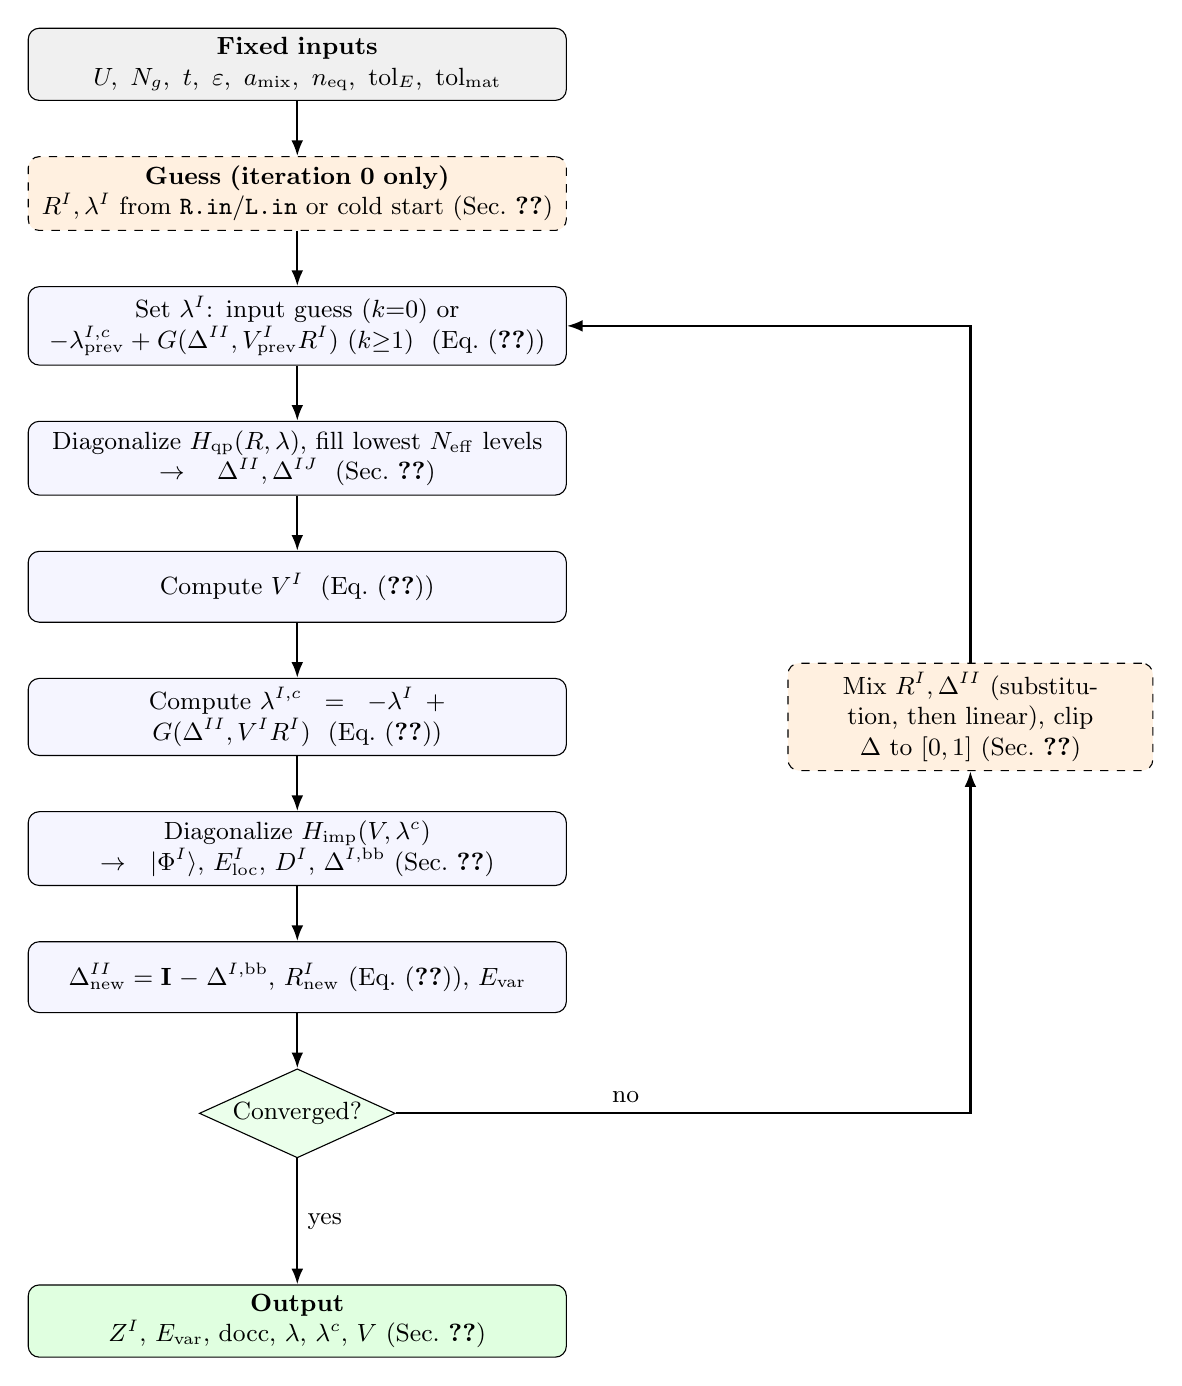
\begin{tikzpicture}[
  node distance=7mm and 14mm,
  box/.style={rectangle, draw, rounded corners, align=center, text width=6.6cm,
              minimum height=9mm, font=\small, fill=blue!4},
  guessbox/.style={box, fill=orange!12, dashed},
  fixedbox/.style={box, fill=gray!12},
  decision/.style={diamond, draw, aspect=2.2, align=center, font=\small,
              inner sep=1pt, fill=green!8},
  outbox/.style={box, fill=green!12},
  arr/.style={-{Latex[length=2mm]}, thick}
]
  \node[fixedbox] (inputs) {\textbf{Fixed inputs}\\ $U,\ \Ng,\ t,\ \varepsilon,\ a_{\mathrm{mix}},\ n_{\mathrm{eq}},\ \mathrm{tol}_E,\ \mathrm{tol}_{\mathrm{mat}}$};
  \node[guessbox, below=of inputs] (guess) {\textbf{Guess (iteration 0 only)}\\ $R^I,\lambda^I$ from \texttt{R.in}/\texttt{L.in} or cold start (Sec.~\ref{sec:cli})};
  \node[box, below=of guess] (lam) {Set $\lambda^I$: input guess ($k{=}0$) or\\ $-\lambda^{I,c}_{\mathrm{prev}}+G(\Delta^{II},V^I_{\mathrm{prev}}R^I)$ ($k{\ge}1$)\ \ (Eq.~\eqref{eq:lambda-update})};
  \node[box, below=of lam] (qp) {Diagonalize $\Hqp(R,\lambda)$, fill lowest $\Neff$ levels\\ $\to\ \Delta^{II},\Delta^{IJ}$ \ (Sec.~\ref{sec:filling})};
  \node[box, below=of qp] (vfit) {Compute $V^I$\ \ (Eq.~\eqref{eq:eqV})};
  \node[box, below=of vfit] (lamc) {Compute $\lambda^{I,c}=-\lambda^I+G(\Delta^{II},V^IR^I)$\ \ (Eq.~\eqref{eq:lambdac-def})};
  \node[box, below=of lamc] (imp) {Diagonalize $\Himp(V,\lambda^c)$\\ $\to\ |\Phi^I\rangle,\,E^I_{\mathrm{loc}},\,D^I,\,\Delta^{I,\mathrm{bb}}$\ (Sec.~\ref{sec:impurity})};
  \node[box, below=of imp] (upd) {$\Delta^{II}_{\mathrm{new}}\!=\!\mathbf I-\Delta^{I,\mathrm{bb}}$,\ $R^I_{\mathrm{new}}$\ (Eq.~\eqref{eq:Rupdate}),\ $E_{\mathrm{var}}$};
  \node[decision, below=of upd] (dec) {Converged?};
  \node[outbox, below=16mm of dec] (out) {\textbf{Output}\\ $Z^I,\,E_{\mathrm{var}},\,\mathrm{docc},\,\lambda,\,\lambda^c,\,V$\ (Sec.~\ref{sec:energy})};
  \node[guessbox, right=28mm of lamc, text width=4.4cm] (newguess) {Mix $R^I,\Delta^{II}$ (substitution, then linear), clip $\Delta$ to $[0,1]$\ (Sec.~\ref{sec:mixing})};

  \draw[arr] (inputs) -- (guess);
  \draw[arr] (guess) -- (lam);
  \draw[arr] (lam) -- (qp);
  \draw[arr] (qp) -- (vfit);
  \draw[arr] (vfit) -- (lamc);
  \draw[arr] (lamc) -- (imp);
  \draw[arr] (imp) -- (upd);
  \draw[arr] (upd) -- (dec);
  \draw[arr] (dec) -- node[right, font=\small]{yes} (out);
  \draw[arr] (dec.east) -| node[pos=0.2, above, font=\small]{no} (newguess.south);
  \draw[arr] (newguess) |- (lam.east);
\end{tikzpicture}
\caption{One outer self-consistency iteration. Gray = fixed for the whole
run. Orange/dashed = a guess or the mixing step. Blue = quantities derived,
in this order. Green = converged output. There is no root-finding step: at
iterations $k\ge1$ the potential $\lambda^I$ is obtained by evaluating
Eq.~\eqref{eq:lambda-update} at the mixed $(R,\Delta)$, and $\Delta^{II}$ is
then \emph{recomputed} from the quasiparticle ground state.}
\label{fig:workflow}
\end{figure}

\section{Specialization to the two-site, two-independent-fragment dimer}
\label{sec:two-fragment}

\subsection{Each site is its own fragment; the two fragments need not be equal}

Each site is treated as its own impurity/fragment. This is the standard gGA
lattice construction applied to a finite two-site ``lattice'': lumping the
whole dimer into a single impurity would leave no inter-site hopping to
renormalize and would make the method vacuous.

\textbf{Important correction relative to an earlier version of this project.}
It is tempting to assume that, because the physical Hamiltonian
Eq.~\eqref{eq:Hphys} is symmetric under exchanging sites $0\leftrightarrow1$,
the two fragments' variational parameters must be equal
($R^0=R^1$, $\lambda^0=\lambda^1$), so that only one impurity problem needs to
be solved per iteration. This is \emph{not} true in general. A reference
calculation for this same dimer at $U/t=2$, $\Ng=2$ converges to a
\emph{genuinely asymmetric} fixed point, with numerically distinct $R^0\neq
R^1$ and $\lambda^0\neq\lambda^1$ (even though $\lvert R^0\rvert\approx\lvert
R^1\rvert$, their components differ substantially -- see
Table~\ref{tab:examples}). The physical dimer's site-exchange symmetry can be
\emph{spontaneously broken} at the level of the auxiliary variational
parameters, exactly as in a mean-field theory with more than one
self-consistent solution. The code therefore \textbf{always} treats the two
fragments as independent variational objects; the possibility that a
converged solution happens to satisfy $R^0=R^1$ is a property of the
solution, never an assumption imposed on the algorithm.

\subsection{Quasiparticle Hamiltonian for two independent fragments}

Let $R^0,R^1\in\mathbb R^{\Neff}$ (column vectors, since $\Nphys=1$) be the two
fragments' renormalization vectors, and $\lambda^0,\lambda^1\in\mathbb
R^{\Neff\times\Neff}$ (real symmetric) their onsite potentials. Because
$\Nphys=1$, the fully general multi-orbital quasiparticle Hamiltonian
\begin{equation}
  \Hqp \;=\; \sum_{I\neq J}\sum_{a,b}\Bigl(\sum_{\alpha,\beta}
     R^{I\dagger}_{a\alpha}\,t^{\alpha\beta}_{IJ}\,R^{J}_{\beta b}
     - \delta_{IJ}\lambda^{I}_{ab}\Bigr) d^{\dagger}_{Ia}d_{Jb}
\end{equation}
collapses, for our two fragments $I,J\in\{0,1\}$ and scalar hopping
$t_{01}=t_{10}=-t$ (with $t^{\alpha\beta}_{IJ}$ having only one value of
$\alpha,\beta$), to the explicit $2\Neff\times2\Neff$ real-space matrix (per
spin channel; both spin channels use the same matrix)
\begin{equation}
  \boxed{\;
  \Hqp \;=\;
  \begin{pmatrix}
    -\lambda^{0} & -t\,R^{0}(R^{1})^{T} \\[2pt]
    -t\,R^{1}(R^{0})^{T} & -\lambda^{1}
  \end{pmatrix}
  \;}
  \label{eq:Hqp2}
\end{equation}
This is the direct generalization of the single-fragment (symmetric) block
matrix $\Hqp=\bigl[\begin{smallmatrix}-\lambda & -tRR^T\\ -tRR^T & -\lambda\end{smallmatrix}\bigr]$
to the case $R^0\neq R^1$, $\lambda^0\neq\lambda^1$; it reduces to the
symmetric form exactly when $R^0=R^1=R$ and $\lambda^0=\lambda^1=\lambda$.
Because there are only two real-space sites, $\Hqp$ is diagonalized directly
(no Brillouin-zone integral is needed, unlike the periodic-lattice
formulation this is specialized from).

\emph{Code:} \texttt{qp\_state(R, lam, t)} builds exactly
Eq.~\eqref{eq:Hqp2} and diagonalizes it with \texttt{numpy.linalg.eigh};
it returns $\Hqp$ and the ground-state 1-RDM $\rho^{\mathrm{qp}}$ of
Section~\ref{sec:filling}.

\subsection{Quasiparticle ground state and occupation rule}
\label{sec:filling}

$\Hqp$ has $2\Neff$ single-particle levels per spin. The quasiparticle
ground state fills a \emph{fixed number} of them. In the reference code the
molecular class (\texttt{RSImpMolecule}, used for \texttt{mol\_type
rsimp\_molecule}) occupies, per spin, the lowest
\begin{equation}
  n_{\mathrm{eff}} \;=\; n_{\mathrm{ph}} + \frac{N_{\mathrm{eff,tot}}-N_{\mathrm{phys,tot}}}{2}
  \;=\; 1+\frac{2\Neff-2}{2} \;=\; \Neff
\end{equation}
eigenvectors of $\Hqp$ (\texttt{mol\_nups}$=n_{\mathrm{ph}}=1$; $N_{\mathrm{eff,tot}}=2\Neff$
quasiparticle orbitals and $N_{\mathrm{phys,tot}}=2$ physical orbitals for the
two fragments). With eigenvalues $\varepsilon_1\le\dots\le\varepsilon_{2\Neff}$ and orthonormal
eigenvectors $|n\rangle$,
\begin{equation}
  \rho^{\mathrm{qp}} \;=\; \sum_{n=1}^{\Neff} |n\rangle\langle n| ,
  \label{eq:rhoqp}
\end{equation}
a fixed \emph{level-count} rule: it does not look at the signs of the
$\varepsilon_n$ and there is no adjustable chemical potential.
The particle-hole symmetric half filling of the physical dimer enters through
the constant $-\mu=-U/2$ contained in $\Hloc$ (Section~\ref{sec:impurity}).

\paragraph{Caution: the base-class rule is different.} The parent class in
the reference code (\texttt{RSImpMod}, used by non-molecular impurity models)
uses instead a zero-temperature Fermi function at chemical potential $0$
(occupy $\varepsilon_n<0$). The two rules coincide whenever $\Hqp$ has exactly
$\Neff$ negative eigenvalues, which is the case at the seeds and at the
converged solutions of the near-converged test cases of
Section~\ref{sec:validation} (there the spectrum is symmetric about zero, e.g.\
$\pm0.0197,\pm0.9375,\pm0.9862$ for the symmetric $U/t=2$ solution), so those
cases cannot tell them apart. Away from self-consistency they do differ: for
example the cold seed $R=(1,1,1)$, $\lambda\approx0$ has eigenvalues
$-2.9995,-0.0002,+7\!\times\!10^{-6},\dots$ with only two negative ones, and
the two rules then give different $\Delta^{11}$. The code follows the
molecular class, i.e.\ Eq.~\eqref{eq:rhoqp}. (An intermediate revision of the
code used the sign rule by mistake, from reading the base class; it was found
by comparing iteration~0 of a cold start with the reference.)

$\rho^{\mathrm{qp}}$ is a $2\Neff\times2\Neff$ matrix; its blocks give the
three independent quasiparticle 1-RDM blocks needed below:
\begin{equation}
  \Delta^{00} = \rho^{\mathrm{qp}}_{[0,\Neff)\times[0,\Neff)},\qquad
  \Delta^{11} = \rho^{\mathrm{qp}}_{[\Neff,2\Neff)\times[\Neff,2\Neff)},\qquad
  \Delta^{01} = \rho^{\mathrm{qp}}_{[0,\Neff)\times[\Neff,2\Neff)} .
  \label{eq:Deltablocks}
\end{equation}
$\Delta^{00}$ and $\Delta^{11}$ are symmetric; $\Delta^{01}$ is in general
\emph{not} symmetric, and $\Delta^{10}=(\Delta^{01})^T$. In the text
$\Delta^{II}$ denotes the fragment-diagonal blocks $\Delta^{00},\Delta^{11}$
and $\Delta^{IJ}$ the off-diagonal one.

\emph{Code:} in \texttt{qp\_state}, \texttt{occ = np.zeros(2*Neff); occ[:Neff] = 1}
implements Eq.~\eqref{eq:rhoqp} (\texttt{eigh} returns ascending eigenvalues), and
\texttt{rho = (evecs * occ) @ evecs.T}.
The blocks of Eq.~\eqref{eq:Deltablocks} are slices of \texttt{rho}
(\texttt{blocks(rho)} in \texttt{run\_gga}, and inside
\texttt{hybridization\_V}).

\section{Self-consistency equations}
\label{sec:selfconsistency}

The gGA self-consistency loop for two fragments couples the quasiparticle side
(Section~\ref{sec:two-fragment}) to an embedding/impurity side through four
fitting/update relations, specialized here from the general multi-fragment
formulation (Mejuto-Zaera, arXiv:2403.05157, Eqs.~5--11) and validated
numerically, block by block, against an independent reference implementation
(see Table~\ref{tab:examples}).

\subsection{Hybridization $V$ (Eq.~7 of the reference)}
\label{sec:eqV}

For fragment $I$, the hybridization vector $V^{I}\in\mathbb R^{\Neff}$ is
fixed by requiring
\begin{equation}
  \sqrt{\Delta^{II}\bigl(\mathbf{I}-\Delta^{II}\bigr)}\;V^{I}
  \;=\; -t\;\Delta^{IJ}\,R^{J}, \qquad J\neq I ,
  \label{eq:eqV}
\end{equation}
i.e.\ for our two fragments,
\begin{align}
  \sqrt{\Delta^{00}(\mathbf{I}-\Delta^{00})}\;V^{0} &= -t\,\Delta^{01}R^{1}, \\
  \sqrt{\Delta^{11}(\mathbf{I}-\Delta^{11})}\;V^{1} &= -t\,(\Delta^{01})^{T}R^{0}.
\end{align}
Notice that $V^{I}$ is fit using the \emph{neighbor} fragment's $R^{J}$ (not
the fragment's own $R^{I}$), and the \emph{cross}-fragment block $\Delta^{IJ}$
(not $\Delta^{II}$). Getting this backwards (using $R^{I}$ instead of
$R^{J}$) is invisible in the symmetric special case $R^0=R^1$ but produces a
completely different, wrong answer once the two fragments differ -- this was
confirmed empirically while developing the code.

The matrix square root in Eq.~\eqref{eq:eqV} is the \emph{shifted} one used by
the reference code,
\begin{equation}
  S(\Delta) \;=\; \sqrt{\Delta(\mathbf I-\Delta)+\varepsilon\,\mathbf I},
  \qquad \varepsilon = 10^{-9}\ \text{(default)},
  \label{eq:Sshift}
\end{equation}
evaluated in the eigenbasis of $\Delta^{II}$: if
$\Delta^{II}=W\,\mathrm{diag}(n_1,\dots,n_{\Neff})\,W^{T}$, then
$S(\Delta^{II})=W\,\mathrm{diag}(s_a)\,W^{T}$ with
$s_a=\sqrt{n_a(1-n_a)+\varepsilon}$, and Eq.~\eqref{eq:eqV} is solved
eigenvalue by eigenvalue,
\begin{equation}
  V^{I} \;=\; W\,\mathrm{diag}\!\left(\frac{1}{s_a}\right)W^{T}\,
    \bigl(-t\,\Delta^{IJ}R^{J}\bigr).
\end{equation}

\paragraph{The shift $\varepsilon$.} At the self-consistent solutions one or
more eigenvalues of $\Delta^{II}$ sit at $0$ or $1$ (a ghost bath orbital
completely empty or completely full). For the symmetric $U/t=2$, $\Ng=2$
solution the eigenvalues of $\Delta^{00}$ are $0$, $\tfrac12$, $1$ to machine
precision, so $n_a(1-n_a)$ is $0$ or a rounding-level number (of either
sign), and the unshifted $1/\sqrt{n_a(1-n_a)}$ is infinite or undefined;
since the corresponding component of the right-hand side is also numerically
zero, the raw formula produces $0/0$ and the whole iteration becomes NaN
(this is what the earlier version of the code did on that case). The
reference code avoids this by adding the shift $\varepsilon$ (input key
\texttt{gg\_sqmat\_shift}) to the \emph{eigenvalues} of $\Delta(\mathbf
I-\Delta)$ before taking the square root (its \texttt{GetMatSqrt(A, regul)}
returns $\sqrt{\text{eigenvalue}+\text{regul}}$) and then solving the linear
system with that matrix; $\Delta$ itself is \emph{not} clipped beforehand.
The code does the same. A component along a direction with $n_a\approx0,1$ is
then $\text{rhs}/\sqrt\varepsilon\sim3\times10^{4}\,\text{rhs}$ with $\text{rhs}$
itself vanishingly small, hence finite, and the value agrees with the
reference. The eigenvalue clip ($10^{-10}$) and the output cap
($V_{\max}=10^{2}$) of the earlier version have been removed: they are not
part of the reference algorithm.

\emph{Code:} \texttt{hybridization\_V(rho, R, t, shift, i)} forms the
right-hand side $-t\,\rho_{ij}R^{J}$ from the blocks of $\rho^{\mathrm{qp}}$
(for fragment $0$: $\Delta^{01}R^1$; for fragment $1$:
$\Delta^{10}R^0=(\Delta^{01})^TR^0$, matching Eq.~\eqref{eq:eqV} exactly,
with the neighbor's $R$) and applies $S(\Delta^{II})^{-1}$ through
\texttt{apply\_S\_inv(Delta, B, shift)}.

\subsection{Bath potential $\lambda^c$ (Eq.~8 of the reference)}
\label{sec:eqlambdac}

The onsite potential $\lambda^{I}$ that enters $\Hqp$
(Eq.~\eqref{eq:Hqp2}) and the bath potential $\lambda^{I,c}$ that enters the
impurity Hamiltonian (Section~\ref{sec:impurity}) are \emph{not} independent
variational parameters. They arise as Lagrange multipliers in the underlying
constrained variational problem, and stationarity of the Lagrangian with
respect to the quasiparticle density matrix $\Delta^{(\mathrm{qp})}$ gives the
linear relation
\begin{equation}
  \lambda^{I}_{ab} + \lambda^{I,c}_{ab}
  \;=\; \left.\frac{\partial}{\partial\Delta^{II}_{ab}}
     \Bigl[R^{I}\cdot\sqrt{\Delta^{II}(\mathbf{I}-\Delta^{II})}\cdot V^{I}\Bigr]\right|_{\mathrm{sym}},
  \label{eq:eqlambdac}
\end{equation}
where $R^{I}$ and $V^{I}$ are held \emph{fixed} in the derivative (i.e.\ $V^I$
is \emph{not} re-substituted through Eq.~\eqref{eq:eqV} as a function of
$\Delta^{II}$ before differentiating), and ``sym'' denotes the standard
symmetric-matrix-gradient convention: for $a=b$ the derivative is taken with
respect to the single diagonal entry, while for $a\neq b$ it is the
\emph{sum} of the two formally independent partial derivatives with respect
to $\Delta_{ab}$ and $\Delta_{ba}$ (equivalently: differentiate along the
symmetric perturbation direction $X_{ab}+X_{ba}$, not along $X_{ab}$ alone,
where $X_{ab}$ denotes the elementary matrix with a $1$ in position $(a,b)$
and $0$ elsewhere -- denoted $X$ rather than the more common $E$ to avoid any
visual clash with the energies $E_{\mathrm{qp}}$, $E^{I,c}$, $E_{\mathrm{loc}}$,
$E_{\mathrm{var}}$ used throughout this document).
Equation~\eqref{eq:eqlambdac} is used to \emph{define} the bath potential
from the current $\lambda^{I}$:
\begin{equation}
  \lambda^{I,c} \;=\; -\lambda^{I} + G\bigl(\Delta^{II},\,V^{I}R^{I}\bigr),
  \label{eq:lambdac-def}
\end{equation}
where $V^I$ is a column, $R^I$ a row, $M=V^IR^I$ is an $\Neff\times\Neff$
matrix, and $G(\Delta,M)$ is the symmetric derivative of the scalar
$S_M(\Delta)=\mathrm{Tr}\bigl[M\,S(\Delta)\bigr]=R\,S(\Delta)\,V$ with respect
to $\Delta$ (with $R,V$ held fixed), in the convention of the reference
code. That convention is: expand in an orthonormal basis $\{B_k\}$ of the real
symmetric $\Neff\times\Neff$ matrices (the generalized Gell-Mann basis,
\texttt{msite\_ggm}; it contains the identity, so it is complete), take the
directional derivative $D_k=\mathrm{d}S[B_k]$ of the matrix square root, and
set
\begin{equation}
  G(\Delta,M) \;=\; \sum_k B_k\;\Bigl(\mathrm{Tr}[M D_k]+\mathrm{Tr}[D_k^{T}M^{T}]\Bigr)
        \;=\; \sum_k B_k\;2\,\mathrm{Tr}[M D_k],
  \label{eq:Gdef}
\end{equation}
(the two traces are equal because $D_k$ is symmetric). Since the basis is
orthonormal, $G$ is twice the projection of the gradient of $S_M$ onto the
symmetric matrices; the factor $2$ is the ``diagonal doubling'' that had to
be found empirically in an earlier version of the code.

\paragraph{Analytic evaluation of $G$.} The derivative of the shifted square
root is available in closed form in the eigenbasis of $\Delta$. Let
$\Delta=W\,\mathrm{diag}(n_a)\,W^T$, $s_a=\sqrt{n_a(1-n_a)+\varepsilon}$,
and use a tilde for quantities in this eigenbasis, $\tilde X=W^TXW$. For a
symmetric perturbation $B$, the derivative of $P=\Delta(\mathbf I-\Delta)$ is
$\mathrm{d}P=B-B\Delta-\Delta B$, i.e.\ $\widetilde{\mathrm{d}P}_{ab}=
\tilde B_{ab}\,(1-n_a-n_b)$. Differentiating $S^2=P+\varepsilon\mathbf I$ gives
the Sylvester equation $S\,\mathrm{d}S+\mathrm{d}S\,S=\mathrm{d}P$, which is
diagonal in this basis:
\begin{equation}
  \widetilde{\mathrm{d}S}_{ab} \;=\; w_{ab}\,\tilde B_{ab},
  \qquad
  w_{ab} \;=\; \frac{1-n_a-n_b}{s_a+s_b}.
\end{equation}
Then $\mathrm{Tr}[M\,\mathrm{d}S[B]]=\sum_{ab}\tilde M_{ba}\,w_{ab}\,\tilde B_{ab}$, and
Eq.~\eqref{eq:Gdef} collapses (summing over the complete orthonormal basis
gives the symmetric part of the coefficient matrix) to
\begin{equation}
  \boxed{\; G(\Delta,M) \;=\; W\Bigl[\bigl(\tilde M+\tilde M^{T}\bigr)\circ w\Bigr]W^{T} \;}
  \label{eq:Gclosed}
\end{equation}
where $\circ$ is the elementwise product. This is exact: it replaces the
central finite-difference evaluation of the earlier version (step
$h=10^{-8}$ on $\sqrt{\Delta(\mathbf I-\Delta)}$ through
\texttt{scipy.linalg.sqrtm}), which is unreliable precisely where it matters,
namely when $\Delta$ has eigenvalues at $0$ or $1$ and $S$ is not
differentiable in the unshifted problem. With the shift, $w_{ab}$ stays
finite for all $a,b$.

\emph{Code:} \texttt{grad\_S(Delta, M, shift)} implements
Eq.~\eqref{eq:Gclosed}; \texttt{embedding\_lambda\_c(Delta, lam, V, R, shift)}
returns $-\lambda+G(\Delta,VR)$, i.e.\ Eq.~\eqref{eq:lambdac-def}.

\subsection{Impurity (embedding) Hamiltonian}
\label{sec:impurity}

For each fragment $I$, the embedding Hamiltonian couples the physical,
interacting orbital (both spins, operators $c_{\uparrow},c_{\downarrow}$) to
$\Neff$ non-interacting bath orbitals per spin (operators
$d_{a\uparrow},d_{a\downarrow}$, $a=1,\dots,\Neff$):
\begin{equation}
  \Himp^{I} \;=\; \Hloc \;+\; \sum_{a=1}^{\Neff}\sum_{\sigma}
    V^{I}_{a}\bigl(d^{\dagger}_{a\sigma}c_{\sigma} + c^{\dagger}_{\sigma}d_{a\sigma}\bigr)
    \;-\; \sum_{a,b=1}^{\Neff}\sum_{\sigma}\lambda^{I,c}_{ab}\,d_{b\sigma}d^{\dagger}_{a\sigma},
  \label{eq:Himp}
\end{equation}
with the local (physical) Hamiltonian, using the \emph{same} $U$ and
particle-hole-symmetric $\mu=U/2$ as the physical dimer,
\begin{equation}
  \Hloc \;=\; U\,n_{\uparrow}n_{\downarrow} \;-\; \mu\,(n_{\uparrow}+n_{\downarrow}), \qquad
  n_\sigma = c^{\dagger}_\sigma c_\sigma .
\end{equation}

\paragraph{Sign of the bath-potential term -- a subtlety.} Equation
\eqref{eq:Himp}'s bath term is written, as it appears in the underlying
Lagrangian, as $-\lambda^{I,c}_{ab}\,d_{b\sigma}d^{\dagger}_{a\sigma}$
(annihilation operator first). This is \emph{not} the same as
$-\lambda^{I,c}_{ab}\,d^{\dagger}_{a\sigma}d_{b\sigma}$: using the fermionic
anticommutator $\{d_{a\sigma},d^{\dagger}_{b\sigma}\}=\delta_{ab}$,
\begin{equation}
  d_{b\sigma}d^{\dagger}_{a\sigma} \;=\; \delta_{ab} - d^{\dagger}_{a\sigma}d_{b\sigma},
\end{equation}
so, dropping the physically irrelevant additive constant $-\sum_{a\sigma}\lambda^{I,c}_{aa}$,
\begin{equation}
  -\sum_{ab\sigma}\lambda^{I,c}_{ab}\,d_{b\sigma}d^{\dagger}_{a\sigma}
  \;\;\widehat{=}\;\;
  +\sum_{ab\sigma}\lambda^{I,c}_{ab}\,d^{\dagger}_{a\sigma}d_{b\sigma} .
  \label{eq:sign-fix}
\end{equation}
The code implements the \emph{right-hand} (normal-ordered, $+$ sign) form of
Eq.~\eqref{eq:sign-fix}. Implementing the naive left-hand form with a
literal $-$ sign in front of $d^{\dagger}_a d_b$ is a sign error that was
present in an earlier version of the code and produced impurity ground-state
energies and 1-RDMs that disagreed with an independent reference
implementation by an order of magnitude; it was found and fixed by comparing
intermediate quantities (bath--bath and bath--impurity blocks of the
impurity 1-RDM) term by term against a reference calculation.

\paragraph{Exact diagonalization via Jordan--Wigner strings.}
\label{sec:JW}
The impurity Hamiltonian, Eq.~\eqref{eq:Himp}, is diagonalized exactly (dense,
full Fock space) using explicit Jordan--Wigner fermion operators. For
$n_{\mathrm{modes}}$ ordered fermionic modes, the annihilation operator for
mode $i$ is
\begin{equation}
  c_i \;=\; Z^{\otimes i}\otimes c_{-}\otimes \mathbf{I}^{\otimes(n_{\mathrm{modes}}-i-1)},
  \qquad
  Z=\begin{pmatrix}1&0\\0&-1\end{pmatrix},\quad
  c_{-}=\begin{pmatrix}0&1\\0&0\end{pmatrix},
  \label{eq:JW}
\end{equation}
acting on the $2^{n_{\mathrm{modes}}}$-dimensional local Fock space, with the
local basis convention $c_{-}|1\rangle=|0\rangle$, $c_{-}|0\rangle=0$
(i.e.\ $(0,1)^{T}$ represents the occupied state). The mode ordering used for
the impurity problem is
\begin{equation}
  0:\ c_{\uparrow},\quad 1:\ c_{\downarrow},\quad
  2{+}2k:\ d_{k\uparrow},\quad 3{+}2k:\ d_{k\downarrow}
  \qquad (k=0,\dots,\Neff-1),
\end{equation}
giving $n_{\mathrm{modes}}=2(1+\Neff)$ total modes and confirming
Eq.~\eqref{eq:fockdim}'s Fock dimension $2^{2(1+\Neff)}=4^{1+\Neff}=4^{2+\Ng}$.
\texttt{exact\_dimer.py} uses the identical Jordan--Wigner construction,
Eq.~\eqref{eq:JW}, for the four physical modes of the full dimer.

\paragraph{Precomputation.} All operator products that do not depend on
$V^{I}$ or $\lambda^{I,c}$ (namely $n_\uparrow$, $n_\downarrow$, $\Hloc$, the
hybridization bilinears $d^\dagger_{a\sigma}c_\sigma+\mathrm{h.c.}$, and the
bath--bath bilinears $d^\dagger_{a\sigma}d_{b\sigma}$) are built \emph{once}
per $(\Neff,U)$ pair (function \texttt{build\_impurity\_ops}), not rebuilt at
every self-consistency iteration; the impurity Hamiltonian for a given
iteration is then simply the weighted sum
$\Himp = \Hloc + \sum_a V_a\,(\text{hyb bilinear})_a + \sum_{ab}\lambda^{c}_{ab}\,(\text{bath bilinear})_{ab}$.
This changes the per-iteration cost from $O(\Neff^2\cdot\dim^3)$ (rebuilding
$\Neff^2$ dense operator products of size $\dim\times\dim$ every iteration) to
$O(\dim^3)$ (one diagonalization), where $\dim=4^{1+\Neff}$; it was the
dominant bottleneck before being fixed.

\paragraph{Ground-state sector.} The reference solver (\texttt{CMZEDsolver})
does not search the whole Fock space. For an even number of impurity orbitals
per spin, $1+\Neff=2+\Ng$ (this is why $\Ng$ must be even), it diagonalizes
$\Himp$ only in the half-filled, spin-balanced sector
$N_\uparrow=N_\downarrow=(1+\Neff)/2$, of dimension
$\binom{1+\Neff}{(1+\Neff)/2}^2$ ($36$ for $\Ng=2$, instead of $256$). The code
does the same: \texttt{build\_impurity\_ops} stores the index set
\texttt{sector} of basis states with these occupations (mode $j$ is occupied
in basis state $i$ iff bit $n_{\mathrm{modes}}-1-j$ of $i$ is set, for the
Jordan--Wigner ordering above) and \texttt{impurity\_solve} diagonalizes
$\Himp[\texttt{sector},\texttt{sector}]$, then embeds the lowest eigenvector back
into the full space so that all expectation values below are unchanged.
This matters far from self-consistency: with the $\lambda^{I,c}$ of an early
cold-start iteration the \emph{global} lowest state of $\Himp$ can lie in
another sector (a triplet, or a different particle number), with a gap to the
half-filled singlet of only $\sim10^{-3}$, and the two solvers then return
different $\Delta^{I,\mathrm{bb}}$ and $D^{I}$. Near convergence the global
ground state is in the sector and the restriction changes nothing.

\paragraph{Hand-over through an FCIDUMP text file.} The reference code does
not pass $V^{I}$ and $\lambda^{I,c}$ to its solver directly: it writes the
embedding Hamiltonian to a text \texttt{FCIDUMP} file
(\texttt{WriteImpFCIDUMP}), each element printed with
\texttt{std::scientific} at precision $12$ (i.e.\ \texttt{\%.12e}), and
\emph{omits} every element with $\lvert x\rvert<10^{-10}$. The solver therefore
sees $V^I$ and $\lambda^{I,c}$ quantized this way. The code reproduces the
quantization (function \texttt{fcidump\_round}, applied to $V^I$ and
$\lambda^{I,c}$ before \texttt{impurity\_solve}; disable with
\texttt{-{}-no-fcidump-rounding}). It is not cosmetic. The $R$ update
$R=S(\Delta_{\mathrm{new}})^{-1}D$ divides by $s_a=\sqrt{n_a(1-n_a)+\varepsilon}$, and at
the cold seeds $\Delta_{\mathrm{new}}$ has eigenvalues within $10^{-8}$--$10^{-16}$
of $1$, so noise well below $10^{-10}$ is amplified into $O(1)$ changes of
$R$. Without the quantization, perturbing a seed by $10^{-12}$ flips the run
between two different fixed points (Section~\ref{sec:validation}); with it the
trajectory is a deterministic function of the seed, as it is in the reference.

\paragraph{Observables.} Given the impurity ground state $|\psi\rangle$
(lowest eigenvector of $\Himp$ in the sector above), all needed expectation values are computed
via matrix--vector products only (never forming $O(\dim\times\dim)$ operator
products explicitly, for the same performance reason):
\begin{align}
  \Delta^{I,\mathrm{bb}}_{ab} &= \tfrac12\Bigl(\langle\psi|d^{\dagger}_{a\uparrow}d_{b\uparrow}|\psi\rangle
     + \langle\psi|d^{\dagger}_{a\downarrow}d_{b\downarrow}|\psi\rangle\Bigr), \\
  D^{I}_{a} &= \tfrac12\Bigl(\langle\psi|d^{\dagger}_{a\uparrow}c_{\uparrow}|\psi\rangle
     + \langle\psi|d^{\dagger}_{a\downarrow}c_{\downarrow}|\psi\rangle\Bigr), \\
  E^{I}_{\mathrm{loc}} &= \langle\psi|\Hloc|\psi\rangle, \qquad
  \mathrm{docc}^{I} = \langle\psi|n_\uparrow n_\downarrow|\psi\rangle, \qquad
  n^{I}_{\mathrm{phys}} = \langle\psi|(n_\uparrow{+}n_\downarrow)|\psi\rangle .
\end{align}
The spin-average in $\Delta^{I,\mathrm{bb}}$ and $D^I$ assumes a paramagnetic
(spin-unpolarized) solution, which is consistent with the fact that $V^I$ and
$\lambda^{I,c}$ enter $\Himp$ identically for both spin channels.

\emph{Code:} \texttt{build\_impurity\_ops(Neff, U, mu)} and
\texttt{impurity\_solve(V, lam\_c, ops)}.

\paragraph{How $D^I$ is actually evaluated.} $D^I_a=\langle\psi|d^\dagger_{a\sigma}c_\sigma|\psi\rangle$
is a \emph{mixed} bath--impurity expectation value, but it is never evaluated
by forming the $\dim\times\dim$ operator product $d^\dagger_ac$ itself.
Instead, since $d_a$ and $c$ are already stored as the elementary
annihilation-operator matrices from Eq.~\eqref{eq:JW}, each is applied
\emph{once} to the ground-state vector $|\psi\rangle$, and the two resulting
vectors are combined with a single inner product:
\begin{equation}
  |u_a\rangle \equiv d_{a\uparrow}|\psi\rangle,\qquad
  |v\rangle \equiv c_\uparrow|\psi\rangle,\qquad
  \langle\psi|d^\dagger_{a\uparrow}c_\uparrow|\psi\rangle \;=\; \langle u_a|v\rangle,
\end{equation}
and likewise for the $\downarrow$ spin channel, with $D^I_a$ the real part of
the spin average of the two. The dagger on $d_a$ is never applied
explicitly: it falls out for free from the conjugate-linearity of the inner
product's first argument (\texttt{numpy.vdot(x, y) = x.conj() @ y}), so
$\langle d_{a\uparrow}\psi|c_\uparrow\psi\rangle=\langle\psi|d^\dagger_{a\uparrow}c_\uparrow|\psi\rangle$
comes out automatically. The bath--bath block $\Delta^{I,\mathrm{bb}}_{ab}$
just above is evaluated the same way, as $\langle u_a|u_b\rangle$ using the
same precomputed $|u_a\rangle$ vectors. This reduces the cost of computing
every observable in Eq.~\eqref{eq:Deltaupdate}--above from $O(\Neff^2\cdot\dim^2)$
(building each mixed operator explicitly, then a matrix--vector product) to
$O(\Neff\cdot\dim)$ for the $\Neff$ vector applications plus $O(\Neff^2)$
cheap inner products -- the same precomputation-driven cost reduction
already noted above for $\Himp$ itself.

\emph{Code:} the vectors \texttt{bu\_gs[a]}, \texttt{bd\_gs[a]},
\texttt{cpu\_gs}, \texttt{cpd\_gs} in \texttt{impurity\_solve}
(\texttt{gga\_dimer.py:591--594}) are exactly $|u_a\rangle$ (both spins) and
$|v\rangle$ (both spins) above; \texttt{D[a] = 0.5*(np.vdot(bu\_gs[a], cpu\_gs)
+ np.vdot(bd\_gs[a], cpd\_gs)).real} (\texttt{gga\_dimer.py:603--607})
implements the formula directly.

\subsection{Update of $R$ and $\Delta$ (Eq.~10 of the reference)}
\label{sec:update}

From the impurity ground state's bath--bath and bath--impurity 1-RDM blocks,
each fragment's target quasiparticle quantities are updated as
\begin{align}
  \Delta^{II,\,\mathrm{new}} &= \mathbf{I} - \Delta^{I,\mathrm{bb}}, \label{eq:Deltaupdate}\\
  \sqrt{\Delta^{II,\mathrm{new}}\bigl(\mathbf{I}-\Delta^{II,\mathrm{new}}\bigr)}\;R^{I,\mathrm{new}} &= D^{I}. \label{eq:Rupdate}
\end{align}
Equation~\eqref{eq:Rupdate} is solved exactly as Eq.~\eqref{eq:eqV}, in the
eigenbasis of $\Delta^{II,\mathrm{new}}$, with the same shifted square root
$S(\Delta^{II,\mathrm{new}})$ of Eq.~\eqref{eq:Sshift}, i.e.
$R^{I,\mathrm{new}}=S(\Delta^{II,\mathrm{new}})^{-1}D^{I}$.

\emph{Code:} \texttt{apply\_S\_inv(Delta\_new, D, shift)}.

\paragraph{Where Eq.~\eqref{eq:Rupdate} comes from.} Equation~\eqref{eq:Rupdate}
is not a new, independent equation -- it is the mirror image of the $V$-fit,
Eq.~\eqref{eq:eqV} (Section~\ref{sec:eqV}). Recall the coupling term of the
Lagrangian, Eq.~\eqref{eq:lagrangian}:
\begin{equation}
  (V^I)^{T}\Bigl[\langle\Phi^I|d^{\dagger}_Ic_I|\Phi^I\rangle
     - \sqrt{\Delta^{II}(\mathbf{I}-\Delta^{II})}\,R^{I}\Bigr] \;+\; \mathrm{h.c.}
\end{equation}
$V^I$ sits there purely as a Lagrange multiplier enforcing that the bracket
vanish. Varying the Lagrangian with respect to $V^I$ itself does not fix a
new value for $V^I$; it simply reinstates the constraint the bracket
represents:
\begin{equation}
  \langle\Phi^I|d^{\dagger}_Ic_I|\Phi^I\rangle
  \;=\; \sqrt{\Delta^{II}(\mathbf{I}-\Delta^{II})}\,R^I,
\end{equation}
which is exactly Eq.~\eqref{eq:Rupdate} once the left-hand side is
identified with $D^I$ (Section~\ref{sec:elderive}, ``Variation with respect
to $R^I$'' explicitly notes that varying with respect to $V^I$, rather than
$R^I$, gives back this $R$-update instead of the $V$-fit). So Eqs.~\eqref{eq:eqV}
and~\eqref{eq:Rupdate} are the \emph{same} underlying relation
$\sqrt{\Delta(\mathbf{I}-\Delta)}\,R=D$-type constraint, solved for different
unknowns at different points of the outer iteration: Eq.~\eqref{eq:eqV}
solves it for $V$ given $R,\Delta$ from the qp side, while
Eq.~\eqref{eq:Rupdate} solves it for $R$ given $D,\Delta$ freshly produced by
the impurity solve.

The $\sqrt{\Delta(\mathbf{I}-\Delta)}$ factor is a coherence weight per bath
direction: an orbital that is essentially empty ($\Delta_{aa}\to0$) or
essentially full ($\Delta_{aa}\to1$) has no partial occupation left to
fluctuate coherently with the physical orbital, so the factor vanishes and
that direction cannot support any $R$ component no matter how large $D_a$
is -- exactly the singular case handled by the shift $\varepsilon$ of
Eq.~\eqref{eq:Sshift}. A half-filled orbital
($\Delta_{aa}=0.5$) has the maximal factor $0.5$ and can carry the most
weight. Eq.~\eqref{eq:Rupdate} is thus best read as: the updated
renormalization amplitude $R^{I}$ is the mixed density $D^I$, rescaled
per bath direction by how much coherent single-particle weight is actually
available in that direction.

\subsection{Variational energy}
\label{sec:energy}

The total variational energy of the two-site lattice, per the general
formula $E_0=\sum_I E^{I}_{\mathrm{imp}} + \sum_{I\neq J}\sum_{ab}
(R^{I\dagger}t_{IJ}R^{J})_{ab}\Delta^{(\mathrm{qp})}_{ab}$ specialized to
$\Nphys=1$, $t_{01}=t_{10}=-t$, and summing the ordered pair $(0,1)$ and
$(1,0)$ contributions (which are equal, since each is the transpose of a
scalar), reads
\begin{equation}
  \boxed{\;
  E_{\mathrm{var}} \;=\; E^{0}_{\mathrm{loc}} + E^{1}_{\mathrm{loc}}
    \;-\; 4t\,\bigl(R^{0}\bigr)^{T}\Delta^{01}R^{1}.
  \;}
  \label{eq:Evar}
\end{equation}
The factor of $4$ combines: a factor $2$ from summing the two ordered
fragment pairs $(I,J)=(0,1)$ and $(1,0)$ (the physical hopping term already
counts the bond once via $c^\dagger_0c_1+\mathrm{h.c.}$, and the ordered-pair
sum over $I\neq J$ reproduces exactly this without double counting), and
another factor $2$ from summing the two spin channels (which contribute
identically under the paramagnetic assumption). $E^{0}_{\mathrm{loc}}+E^{1}_{\mathrm{loc}}$
(not $2E_{\mathrm{loc}}$) is used because the two fragments' impurity
ground states are, in general, different.

At $U=0$, for any $\Ng$, the code reproduces $E_{\mathrm{var}}=-2t$ exactly
(the exact, uncorrelated dimer answer), which is used throughout as a hard
consistency check on Eq.~\eqref{eq:Evar} and on every other formula that
feeds into it.

\section{Numerical solution of the self-consistency loop}
\label{sec:outer-loop}

Sections~\ref{sec:eqV}--\ref{sec:update} define, for a \emph{given}
$(R^0,R^1,\lambda^0,\lambda^1)$, how to compute
$\Delta^{00},\Delta^{11},\Delta^{01}$ (Section~\ref{sec:two-fragment}),
$V^0,V^1$ (Section~\ref{sec:eqV}), $\lambda^{0,c},\lambda^{1,c}$
(Section~\ref{sec:eqlambdac}), the impurity solve
(Section~\ref{sec:impurity}), and the updated
$R^{I}_{\mathrm{new}},\Delta^{II}_{\mathrm{new}}$
(Section~\ref{sec:update}). What remains is (a) how $\lambda^I$ is produced at
each outer iteration, and (b) how the iteration over $(R,\Delta)$ is driven to
a fixed point. As stated in Section~\ref{sec:workflow}, both follow the
reference C++ code exactly.

\subsection{Where $\lambda^I$ comes from: no fit, just Eq.~\eqref{eq:eqlambdac}}
\label{sec:lambdafit}

At iteration $0$, $\lambda^I$ is the input guess and $\Delta^{II}$ is simply
the block of the quasiparticle ground state $\rho^{\mathrm{qp}}(R,\lambda)$
built from it. At every later iteration $k\ge1$, $\lambda^I$ is obtained by
solving the stationarity condition Eq.~\eqref{eq:eqlambdac} for $\lambda^I$,
using the previous iteration's bath potential and hybridization and the
current (mixed) $R^I$ and $\Delta^{II}$:
\begin{equation}
  \lambda^{I}_{k} \;=\; -\lambda^{I,c}_{k-1} \;+\; G\bigl(\Delta^{II}_{k},\,V^{I}_{k-1}R^{I}_{k}\bigr).
  \label{eq:lambda-update}
\end{equation}
Then $\Hqp(R_k,\lambda_k)$ is diagonalized and $\Delta^{II}_k,\Delta^{IJ}_k$ are
\emph{recomputed} from its ground state, Eq.~\eqref{eq:rhoqp}; $V^I_k$
(Eq.~\eqref{eq:eqV}) and $\lambda^{I,c}_k$ (Eq.~\eqref{eq:lambdac-def}) follow
from these. Note the consequences:
\begin{itemize}
  \item the mixed $\Delta^{II}$ carried between iterations enters only through
    $G$ in Eq.~\eqref{eq:lambda-update}; the $\Delta^{II}$ used for $V$,
    $\lambda^c$ and the energy is the one produced by $\Hqp$, so the equality
    of the quasiparticle and impurity density matrices,
    $\Delta^{II}_{\mathrm{qp}}=\Delta^{II}_{\mathrm{new}}$, holds only at
    self-consistency (this is the constraint of the $\lambda^I$-term of the
    Lagrangian, Section~\ref{sec:lagrangian});
  \item nothing is solved iteratively inside an outer iteration: each step is
    a closed-form evaluation plus two diagonalizations of small matrices and
    two impurity solves, so there is no branch ambiguity to control.
\end{itemize}

\paragraph{What this replaces.} An earlier version of the code instead
\emph{fitted} $(\lambda^0,\lambda^1)$ at every iteration by a damped Newton
solve (analytic Jacobian of the projector $\rho^{\mathrm{qp}}$, trust-region
step cap, line search) so that the qp density matrix
reproduced a target $\Delta$, the mixed impurity result. That is the
reference code's \emph{other} branch (\texttt{no\_fit\_scf F}, routine
\texttt{OptLambd}); it is a different algorithm from the one the reference
runs used here (\texttt{no\_fit\_scf T}), and on the reference seeds it
diverged: the target $\Delta$ coming from the impurity is generally not
reachable by the qp problem at fixed $R$, so the fit walked away from the
physical branch (e.g.\ the physical filling drifted to
$n_{\mathrm{phys}}\approx1.02$ and then $1.28$ within three iterations on the
$U/t=2$ seed). The fit machinery, the DIIS mixer, the ``best iterate''
safety net and the gauge-fixing routine were all removed together with this;
the fit branch is not implemented.

\subsection{Outer loop: mixing and convergence}
\label{sec:mixing}

After the impurity solves one has, per fragment, $\Delta^{II}$ and $R^I$
(current) and $\Delta^{II}_{\mathrm{new}}$, $R^I_{\mathrm{new}}$
(Section~\ref{sec:update}). The reference \texttt{lin} updater then forms
\begin{equation}
  X_{\mathrm{next}} \;=\; X + a_k\,\bigl(X_{\mathrm{new}}-X\bigr),\qquad
  X\in\{R^0,R^1,\Delta^{00},\Delta^{11}\},
  \qquad
  a_k=\begin{cases}1 & k_{\mathrm{upd}}\le n_{\mathrm{eq}}\\
                    a_{\mathrm{mix}} & k_{\mathrm{upd}}>n_{\mathrm{eq}}\end{cases}
  \label{eq:linmix}
\end{equation}
where $k_{\mathrm{upd}}=1,2,\dots$ counts the calls of the mixer. That is,
\emph{plain substitution} during the first $n_{\mathrm{eq}}$ iterations
(\texttt{gg\_eq\_time}, default $10$), then linear mixing with weight
$a_{\mathrm{mix}}$ (\texttt{gg\_lin\_mix}, default $0.65$). The eigenvalues of
each $\Delta^{II}_{\mathrm{next}}$ are then clipped to $[0,1]$ (the reference
\texttt{reg\_mat} step; the clip is applied to the mixed matrix, not to the
$\Delta$ that enters $S$).

\paragraph{Convergence test.} With $E^{(k)}_{\mathrm{var}}$ the variational
energy of iteration $k$ (Eq.~\eqref{eq:Evar}), define
\begin{align}
  \delta E_k &= E^{(k)}_{\mathrm{var}}-E^{(k-1)}_{\mathrm{var}}
     \quad(E^{(-1)}_{\mathrm{var}}\equiv100),\\
  \delta\Delta_k &= \sum_{I}\bigl\lVert\Delta^{II}_{\mathrm{next},k-1}-\Delta^{II}_{\mathrm{next},k}\bigr\rVert_F
     \quad(\Delta_{\mathrm{next},-1}\equiv\text{the qp block at iteration }0),\\
  \delta R_k &= \sum_{I}\bigl\lVert R^{I}_{k}-R^{I}_{\mathrm{next},k}\bigr\rVert ,
\end{align}
the sum running over the two fragments. The loop stops when
$\lvert\delta E_k\rvert<\mathrm{tol}_E$ \emph{or}
($\delta\Delta_k<\mathrm{tol}_{\mathrm{mat}}$ \emph{and}
$\delta R_k<\mathrm{tol}_{\mathrm{mat}}$); the defaults are
$\mathrm{tol}_E=\mathrm{tol}_{\mathrm{mat}}=10^{-6}$, the reference values
(\texttt{gg\_abs\_tol\_E}, \texttt{gg\_abs\_tol\_mat}). The maximum number of
iterations defaults to $200$. Nothing is returned other than the last
iteration (there is no ``best iterate'' selection).

\paragraph{Reported state.} At return, $R^I$ is the \emph{updated} $R$ after the
last mixing step (the C++ \texttt{final\_R}), $\lambda^I$, $\lambda^{I,c}$,
$V^I$, $E_{\mathrm{var}}$, $\mathrm{docc}$ and $n_{\mathrm{phys}}$ are those of
the last iteration.

\emph{Code:} \texttt{run\_gga(Ng, U, t=1.0, max\_iter=200, tol\_E=1e-6,
tol\_mat=1e-6, mix=0.65, eq\_time=10, sqmat\_shift=1e-9, verbose=False,
Rg0=None, Rg1=None, lamg0=None, lamg1=None)}. \texttt{Rg1}/\texttt{lamg1}
default to \texttt{Rg0}/\texttt{lamg0} when not given; if nothing is given at
all, $R^0=(0.9,\,0.05,\,0.05\cdot1.3,\,0.05\cdot1.6,\dots)$ (distinct ghost
components, to break the exact ghost-exchange symmetry) and $\lambda^0=0$
(the C++ default is $R=(1,\dots,1)$, $\lambda=0$).

\subsection{The main self-consistency loop, in pseudocode}
\label{sec:mixing-algo}

\begin{lstlisting}[language=Python]
def run_gga(Ng, U, t=1.0, max_iter=200, tol_E=1e-6, tol_mat=1e-6,
            mix=0.65, eq_time=10, sqmat_shift=1e-9,
            Rg0=None, Rg1=None, lamg0=None, lamg1=None):
    Neff = 1 + Ng
    ops = build_impurity_ops(Neff, U, U / 2.0)      # precomputed once
    R, lam = seeds(Rg0, Rg1, lamg0, lamg1)          # lists [frag0, frag1]
    lamc = [0, 0]; V = [0, 0]; curr_E = 100.0; n_upd = 0

    for it in range(max_iter):
        if it == 0:
            Hqp, rho = qp_state(R, lam, t)          # lam = input guess
            Delta = blocks(rho); prev_Delta = Delta
        else:                                       # Eq. (lambda-update)
            lam = [-lamc[i] + grad_S(Delta[i], outer(V[i], R[i]), eps)
                   for i in (0, 1)]
            Hqp, rho = qp_state(R, lam, t)
            Delta = blocks(rho)                     # recomputed from Hqp

        V    = [hybridization_V(rho, R, t, eps, i) for i in (0, 1)]   # Eq. (V)
        lamc = [-lam[i] + grad_S(Delta[i], outer(V[i], R[i]), eps)
                for i in (0, 1)]                                       # Eq. (lamc)

        imp = [impurity_solve(V[i], lamc[i], ops) for i in (0, 1)]   # ED
        Delta_new = [I - imp[i].Delta_bb for i in (0, 1)]             # Eq. (Delta)
        R_new     = [S_inv(Delta_new[i]) @ imp[i].D for i in (0, 1)]  # Eq. (R)

        E_var = 2*trace(rho @ (Hqp + blockdiag(lam))) + Eloc0 + Eloc1 # Eq. (Evar)

        n_upd += 1;  a = 1.0 if n_upd <= eq_time else mix             # Eq. (linmix)
        Delta_next = [Delta[i] + a*(Delta_new[i] - Delta[i]) for i in (0, 1)]
        R_next     = [R[i]     + a*(R_new[i]     - R[i])     for i in (0, 1)]
        Delta_next = [clip_eigenvalues(D, 0, 1) for D in Delta_next]

        dD = sum(norm(prev_Delta[i] - Delta_next[i]) for i in (0, 1))
        dR = sum(norm(R[i] - R_next[i])              for i in (0, 1))
        dE = E_var - curr_E
        prev_Delta, R, Delta, curr_E = Delta_next, R_next, Delta_next, E_var
        if abs(dE) < tol_E or (dD < tol_mat and dR < tol_mat):
            break
    return R, lam, lamc, V, E_var, ...              # last iteration
\end{lstlisting}

\subsection{Validation against the reference C++ code, iteration by iteration}
\label{sec:validation}

The reference code writes, for every iteration, the intermediate quantities
(\texttt{curr\_deltas}, \texttt{curr\_Vs}, \texttt{curr\_lambdcs},
\texttt{imp\_1rdms}, \texttt{new\_Rs}, $E_{\mathrm{var}}$, $\delta\Delta$,
$\delta R$) to \texttt{gg.out}. Two $U/t=2$, $\Ng=2$ test cases, differing only
in the seed $(R,\lambda)$ read from the reference \texttt{guess\_*.dat}
files, were run with both codes: \texttt{backward} (a generic, asymmetric seed
with $\Delta$-eigenvalues $3.5\times10^{-5},\tfrac12,0.99996$) and
\texttt{forward} (the symmetric-solution seed with $\Delta$-eigenvalues
exactly $0,\tfrac12,1$, the one that produced NaN before the shift was
introduced). The results agree at every step:
\begin{table}[h]
\centering
\small
\begin{tabular}{crrrrrr}
\toprule
 & \multicolumn{2}{c}{$E_{\mathrm{var}}/t$} & \multicolumn{2}{c}{$\delta\Delta$} & \multicolumn{2}{c}{$\delta R$} \\
\cmidrule(lr){2-3}\cmidrule(lr){4-5}\cmidrule(lr){6-7}
$k$ & this code & C++ & this code & C++ & this code & C++ \\
\midrule
0 & $-3.113524$ & $-3.11352$ & $3.998\!\times\!10^{-4}$ & $3.998\!\times\!10^{-4}$ & $2.396\!\times\!10^{-2}$ & $2.396\!\times\!10^{-2}$ \\
1 & $-3.124827$ & $-3.12483$ & $4.121\!\times\!10^{-4}$ & $4.121\!\times\!10^{-4}$ & $1.665\!\times\!10^{-3}$ & $1.665\!\times\!10^{-3}$ \\
2 & $-3.125596$ & $-3.12560$ & $3.098\!\times\!10^{-5}$ & $3.098\!\times\!10^{-5}$ & $1.270\!\times\!10^{-4}$ & $1.270\!\times\!10^{-4}$ \\
3 & $-3.125656$ & $-3.12566$ & $2.458\!\times\!10^{-6}$ & $2.458\!\times\!10^{-6}$ & $1.009\!\times\!10^{-5}$ & $1.009\!\times\!10^{-5}$ \\
4 & $-3.125661$ & $-3.12566$ & $1.964\!\times\!10^{-7}$ & $1.964\!\times\!10^{-7}$ & $8.063\!\times\!10^{-7}$ & $8.063\!\times\!10^{-7}$ \\
\bottomrule
\end{tabular}
\caption{Iteration-by-iteration comparison, \texttt{backward} case
($U/t=2$, $\Ng=2$). The C++ $E_{\mathrm{var}}$ is printed with six
significant figures in its log.}
\label{tab:cppcompare}
\end{table}

For \texttt{forward}, $E_{\mathrm{var}}$ goes $-3.136429,\,-3.125710,\,
-3.125044,\,-3.125003,\,-3.125000$ (C++: $-3.13643,\,-3.12571,\,-3.12504,\,
-3.12500,\,-3.12500$) and $\delta R$ goes $5.892\!\times\!10^{-3},\,
3.665\!\times\!10^{-4},\,2.290\!\times\!10^{-5},\,1.431\!\times\!10^{-6},\,
8.950\!\times\!10^{-8}$ (C++: the same to the printed digits); in this case
$\delta\Delta$ is at the rounding level ($\sim10^{-9}$--$10^{-10}$) in both
codes after the first iteration, so only its order of magnitude is
meaningful. The final quasiparticle weight is $Z=0.9375$ ($=$ the
eigenvalue of $R^\dagger R$ printed by the C++ code). In both cases the
final $R$ and $\lambda$ written by \texttt{save\_results} agree with the C++
\texttt{final\_R\_*.dat} and \texttt{final\_lambda\_*.dat} to
$\lesssim10^{-9}$ in every entry, and both runs converge in $5$
iterations, as in the reference.

\paragraph{Cold starts.} The reference code has no built-in initial guess:
it reads $R$ and $\lambda$ from files. To test cold starts, the same seed files
were given to both codes: $R=(1,1,1)$ (``ones''), the code's default
$R=(0.9,0.05,0.065)$ (``pydef''), and a random $R\in[0.05,1]^3$
(``rand1''), each with $\lambda=0$, plus ``onesN'' and ``pydefN'' which add the
same small symmetric random $\lambda$ ($\sim10^{-3}$) to break the exact
degeneracy of $\Hqp$ at $\lambda=0$; $U/t\in\{2,4,8,10\}$, $\Ng=2$. Result:
\emph{all $20$ runs converge with both codes, and the iteration counts and
final $Z$ are identical in all $20$} (energies agree to the digits the C++ log
prints):
\begin{table}[h]
\centering
\small
\begin{tabular}{lrrrr}
\toprule
seed & $U/t=2$ & $U/t=4$ & $U/t=8$ & $U/t=10$ \\
\midrule
ones   & $-3.1250$ (8)  & $-4.5000$ (12) & $-8.0001$ (189) & $-10.0000$ (35) \\
pydef  & $-3.1250$ (7)  & $-4.5000$ (11) & $-8.0001$ (187) & $-10.0000$ (34) \\
rand1  & $-3.1250$ (7)  & $-4.5000$ (11) & $-8.0001$ (188) & $-10.0000$ (34) \\
onesN  & $-3.1257$ (7)  & $-4.5111$ (15) & $-8.1276$ (33)  & $-10.1013$ (16) \\
pydefN & $-3.1257$ (7)  & $-4.5111$ (12) & $-8.1276$ (23)  & $-10.1013$ (15) \\
\bottomrule
\end{tabular}
\caption{Final $E_{\mathrm{var}}/t$ (number of iterations) from cold seeds,
$\Ng=2$; the C++ code gives the same numbers. Exact energies: $-3.2361$,
$-4.8284$, $-8.4721$, $-10.3852$.}
\label{tab:cold}
\end{table}

\paragraph{Reading Table~\ref{tab:cold}.} The fixed-point map has several
solutions (as in any mean-field-like variational theory), and which one a cold
start reaches depends on the seed, in the \emph{same} way for both codes. With
$\lambda=0$ the seed sits on an exactly symmetric manifold and the run
falls onto the plain-Gutzwiller branch: $Z=0.75$, $E=-4.5$ at $U/t=4$, and
$Z\approx5\!\times\!10^{-6}$, $E=-10$ at $U/t=10$, i.e.\ the ghost orbitals stay
unused ($\Ng=0$ gives the same values). With a tiny $\lambda$ noise the run
finds the ghost-assisted solution ($E=-4.5111$, $-8.1276$, $-10.1013$, the same
as the seeded examples), which is lower in energy and closer to the exact
values, so a cold start does \emph{not} guarantee the best solution: at
$\lambda=0$ both codes converge, but to a higher-energy branch. Seeding
\texttt{R.in}/\texttt{L.in} from a good solution, or a small random $\lambda$,
is the reliable way to reach the lower branch.

\paragraph{Sensitivity, and why the FCIDUMP quantization is emulated.} At
$U/t=10$ the reference code's $\lambda=0$ run ends on the localized branch
($E=-10$), whereas the code without the FCIDUMP quantization
of Section~\ref{sec:impurity}, with seed perturbations of only $10^{-12}$, lands
on either branch depending on the perturbation ($E=-10.1013$ for some, $-10.0000$
for others), while the reference code gives $E=-10$ for all six perturbed
seeds. With the quantization emulated the code gives $E=-10.0000$ in all six, in
$34$ iterations like the reference (and $188$ iterations, $Z=0.007935$ at
$U/t=8$, again as the reference).

\section{Observables reported by the code}

\begin{itemize}
  \item \textbf{Quasiparticle weight} $Z^{I}=\lVert R^{I}\rVert^2=(R^I)^TR^I$,
    reported per fragment as \texttt{Z0}, \texttt{Z1}.
  \item \textbf{Variational energy} $E_{\mathrm{var}}$, Eq.~\eqref{eq:Evar}.
  \item \textbf{Double occupancy} $\mathrm{docc}=\tfrac12(\mathrm{docc}^0+\mathrm{docc}^1)$,
    the fragment-averaged impurity double occupancy (Section~\ref{sec:impurity}),
    directly comparable to \texttt{exact\_dimer.py}'s \texttt{docc/site} column.
  \item \textbf{Physical filling} $n_{\mathrm{phys}}=\tfrac12(n^0_{\mathrm{phys}}+n^1_{\mathrm{phys}})$.
  \item \textbf{Final parameters} $R^0,R^1,\lambda^0,\lambda^1,\lambda^{0,c},
    \lambda^{1,c},V^0,V^1$ of the last iteration ($R$ after the last mixing
    step, as in the reference), all returned in the result dictionary
    (together with a \texttt{converged} flag) and, from
    the command line, written to \texttt{<prefix>\_R.dat},
    \texttt{<prefix>\_lambda.dat}, \texttt{<prefix>\_lambda\_c.dat} (one
    row-block per fragment: atom~0 then atom~1).
  \item \textbf{Spectral function} $A(\omega)$ (Section~\ref{sec:spectral}),
    computed only if \texttt{-{}-omega}, \texttt{-{}-eta}, \texttt{-{}-domega}
    are given, written to \texttt{A\_omega.txt}.
\end{itemize}

\section{Post-processing: quasiparticle Green's function and spectral function}
\label{sec:spectral}

Once the outer loop of Section~\ref{sec:outer-loop} has converged, the same
converged $\Hqp(R^0,R^1,\lambda^0,\lambda^1)$ (Eq.~\eqref{eq:Hqp2}) can
optionally be reused, as a cheap post-processing step, to evaluate the
one-body quasiparticle Green's function and, from it, the physical spectral
function of the dimer. This is a diagnostic/plotting step only: it does not
feed back into the self-consistency loop.

\paragraph{Quasiparticle Green's function.} On a uniform real-frequency grid
running from $-\omega_{\max}$ to $+\omega_{\max}$ in steps of
$d\omega$ (all three, $\omega_{\max}$, the broadening $\eta$, and $d\omega$,
are supplied by the user -- Section~\ref{sec:cli}), the $2\Neff\times2\Neff$
retarded quasiparticle Green's function is
\begin{equation}
  G(\omega) \;=\; \bigl[(\omega+i\eta)\,\mathbf{I} - \Hqp\bigr]^{-1},
  \label{eq:Gqp}
\end{equation}
with $\Hqp$ the same fixed, converged matrix of Eq.~\eqref{eq:Hqp2} (the
same one for both spin channels, since $\Hqp$ does not carry a spin index)
and $\mathbf I$ here the $2\Neff\times2\Neff$ identity.

\paragraph{Transformation to the physical basis.} The physical creation
operator of fragment $I$ is related to the qp/bath operators by
$c^{\dagger}_I\to\sum_a R^I_a d^{\dagger}_{Ia}$ (Eq.~14 of
\texttt{NotesOngGut.pdf}, already used in Section~\ref{sec:lagrangian}).
Collecting both fragments' $R$ vectors into a single block-diagonal
$2\Neff\times2$ matrix,
\begin{equation}
  R_{\mathrm{mat}} \;=\; \begin{pmatrix} R^0 & 0 \\ 0 & R^1 \end{pmatrix}
  \in\mathbb R^{2\Neff\times2},
\end{equation}
the $2\times2$ physical-basis (site-resolved) Green's function is the
congruence transform
\begin{equation}
  G_{\mathrm{phys}}(\omega) \;=\; R_{\mathrm{mat}}^{T}\,G(\omega)\,R_{\mathrm{mat}} ,
  \label{eq:Gphys}
\end{equation}
whose diagonal entries are the site-0/site-1 physical Green's functions and
whose off-diagonal entries are the inter-site physical Green's function
mediated by the qp sector.

\paragraph{Spectral function.} Tracing Eq.~\eqref{eq:Gphys} sums the two
sites' contributions; the total physical spectral function is
\begin{equation}
  \boxed{\;A(\omega) \;=\; -\frac{2}{\pi}\,\mathrm{Im}\,\mathrm{Tr}\bigl[G_{\mathrm{phys}}(\omega)\bigr]\;}
  \label{eq:Aomega}
\end{equation}
The factor of $2$ accounts for both spin channels: $\Hqp$, and hence $G(\omega)$
and $G_{\mathrm{phys}}(\omega)$, is identical for $\uparrow$ and $\downarrow$
(the paramagnetic solutions this code targets never distinguish them), so
the total spectral weight is twice the single-spin trace computed from
Eq.~\eqref{eq:Gqp}--\eqref{eq:Gphys}.

\paragraph{Sum rule (validation).} For a normalized single-particle Green's
function, $\int_{-\infty}^{\infty}A(\omega)\,d\omega$ must equal the total
number of physical (site, spin) degrees of freedom, i.e.\ $2$ sites $\times$
$2$ spins $=4$. Numerically integrating $A(\omega)$ from
\texttt{examples/Ng2\_U10} ($U/t=10$, $\Ng=2$) over $\omega\in[-15,15]$ with
$\eta=0.05$, $d\omega=0.05$ gives $\int A\,d\omega\approx3.96$, within the
expected error from the finite frequency cutoff and the Lorentzian
broadening tails that extend (slightly) past $\pm\omega_{\max}$ -- confirming
both the overall normalization and the factor of $2$ in
Eq.~\eqref{eq:Aomega}.

\emph{Code:} \texttt{compute\_spectral\_function(R0, R1, lam0, lam1, t,
omega\_max, eta, domega)} builds $\Hqp$ and $R_{\mathrm{mat}}$ once, then
loops over the frequency grid (built with \texttt{numpy.arange} padded by
half a step so the closed endpoint $+\omega_{\max}$ survives floating-point
round-off) evaluating Eqs.~\eqref{eq:Gqp}--\eqref{eq:Aomega} at each point;
\texttt{save\_spectral\_function} writes the two-column result
(\texttt{omega}, \texttt{A(omega)}) to \texttt{A\_omega.txt}.

\section{Command-line interface and input file formats}
\label{sec:cli}

\begin{lstlisting}[language=bash]
python3 gga_dimer.py --U <U/t> --Ng <even integer>
                      [--t <hopping, default 1.0>]
                      [--max-iter <default 200>]
                      [--sqmat-shift <default 1e-9>]
                      [--no-fcidump-rounding]
                      [--mix <default 0.65>] [--eq-time <default 10>]
                      [--tol-E <default 1e-6>] [--tol-mat <default 1e-6>]
                      [--quiet]
                      [--R-file <path, default R.in>]
                      [--lam-file <path, default L.in>]
                      [--omega <omega_max> --eta <eta> --domega <step>]
\end{lstlisting}
The last five numerical options correspond one to one to the reference input
keys \texttt{gg\_sqmat\_shift}, \texttt{gg\_lin\_mix}, \texttt{gg\_eq\_time},
\texttt{gg\_abs\_tol\_E} and \texttt{gg\_abs\_tol\_mat} (and \texttt{-{}-max-iter}
to \texttt{gg\_maxits}); \texttt{-{}-no-fcidump-rounding} switches off the
emulation of the reference FCIDUMP hand-over of Section~\ref{sec:impurity}. The option \texttt{-{}-regularize} of the earlier
version no longer exists (the clips and caps it switched on are not part of
the reference algorithm). Called with no \texttt{-{}-U}/\texttt{-{}-Ng}, the
script instead prints a default sweep over $\Ng\in\{0,2,4\}$ and
$U/t\in\{0,1,2,4,8\}$, using the default cold-start seed for every point (no
external guess files are read in this mode).

\paragraph{\texttt{-{}-omega}, \texttt{-{}-eta}, \texttt{-{}-domega}.} Optional,
and only meaningful together with \texttt{-{}-U}/\texttt{-{}-Ng}; the three
must be given together (any one given without the other two is a CLI error).
When given, after the self-consistency loop converges the code evaluates the
spectral function of Section~\ref{sec:spectral} on the grid
$-\texttt{omega}$ to $+\texttt{omega}$ in steps of \texttt{domega}, with
broadening \texttt{eta}, and writes \texttt{A\_omega.txt} in the current
directory. None of the three has a default: the user must supply all three
explicitly, since there is no physically motivated default frequency window,
broadening, or resolution -- these depend entirely on the energy scales
($U$, $t$, the converged $\lambda,\lambda^c$) of the particular run.

\paragraph{\texttt{R.in}.} Either \emph{one} row of $\Neff$ numbers
(used as a symmetric guess, $R^0=R^1=$ that row) or \emph{two} rows of
$\Neff$ numbers each (fragment $0$'s row, then fragment $1$'s row), free-format
whitespace- or comma-separated.

\paragraph{\texttt{L.in}.} Either $\Neff$ rows of $\Neff$ numbers (one
symmetric matrix, used for both fragments) or $2\Neff$ rows of $\Neff$
numbers (fragment $0$'s $\Neff\times\Neff$ block, stacked on top of fragment
$1$'s block), free-format. To seed a run from the reference C++ code's
\texttt{guess\_L1.dat}, \texttt{guess\_L2.dat} (one $\Neff\times\Neff$ matrix per
fragment) and \texttt{guess\_R1.dat}, \texttt{guess\_R2.dat} (one row per
fragment), simply concatenate them: $\texttt{L.in}=\texttt{guess\_L1.dat}$ then
$\texttt{guess\_L2.dat}$, and likewise for \texttt{R.in}.

Both files are read automatically if present in the working directory (or at
the path given by \texttt{-{}-R-file}/\texttt{-{}-lam-file}); if absent, the
default cold-start seed of Section~\ref{sec:mixing} is used. Every run
writes its final $(R,\lambda,\lambda^c)$ back out in exactly this stacked,
two-row-block format (\texttt{save\_results}), so a converged run's output
can be fed back in directly as the next run's guess.

\section{Worked examples and current validation status}
\label{sec:examples}

Two examples, seeded from an independent reference implementation's own
iterates, are kept under \texttt{examples/}. In addition, the two
reference test cases of Section~\ref{sec:validation} (\texttt{forward} and
\texttt{backward}, with the reference code's complete \texttt{gg.out} logs)
are the primary, iteration-by-iteration validation of everything in this
document.

\begin{table}[h]
\centering
\begin{tabular}{lccccc}
\toprule
Example & $\Ng$ & $U/t$ & seed type & this code's $E_{\mathrm{var}}/t$ & reference $E_{\mathrm{var}}/t$ \\
\midrule
\texttt{examples/Ng2\_U10} & 2 & 10 & symmetric ($R^0{=}R^1$) & $-10.101314$ & $-10.101316$ \\
\texttt{examples/Ng2\_U2}  & 2 & 2  & asymmetric ($R^0{\neq}R^1$) & $-3.125661$ & $-3.12566$ \\
\texttt{forward} (Sec.~\ref{sec:validation})  & 2 & 2  & symmetric-solution seed & $-3.125000$ & $-3.125$ \\
\bottomrule
\end{tabular}
\caption{Seeded reference examples and the agreement obtained with the
algorithm of Section~\ref{sec:outer-loop} (the \texttt{backward} case is
the same physical solution as \texttt{examples/Ng2\_U2}, Table~\ref{tab:cppcompare}).}
\label{tab:examples}
\end{table}

\section{References}
\label{sec:refs}

\begin{enumerate}
  \item N. Lanat\`a \emph{et al.}, ``Phase Diagram and Electronic Structure
    of Praseodymium and Plutonium,'' Phys. Rev. X \textbf{5}, 011008 (2015);
    and N. Lanat\`a \emph{et al.}, Phys. Rev. X \textbf{7}, 031013 (2017) --
    original ghost Gutzwiller approximation.
  \item F. Mejuto-Zaera and M. Fabrizio, ``Efficient computational screening
    of strongly correlated materials: Multi-orbital phenomenology within the
    ghost Gutzwiller approximation,'' arXiv:2305.03329 -- procedural
    formulation for periodic lattices (source of the general $\Hqp$,
    filling, and update-equation structure specialized in
    Section~\ref{sec:two-fragment}).
  \item F. Mejuto-Zaera, ``Quantum embedding for molecules using auxiliary
    particles -- the ghost Gutzwiller ansatz,'' Faraday Discuss. \textbf{254},
    653 (2024), arXiv:2403.05157 -- finite/molecular (non-periodic)
    formulation; the direct source of Eqs.~\eqref{eq:eqV}--\eqref{eq:Evar}
    (Eqs.~7--11 of that paper) as specialized here to the two-site,
    two-independent-fragment dimer.
  \item C. Mejuto-Zaera, ``Notes on (ghost) Gutzwiller'' (unpublished notes,
    \texttt{NotesOngGut.pdf}) -- the source of the Lagrangian derivation
    underlying Eq.~\eqref{eq:eqlambdac} (its Eq.~29) and of the impurity
    Hamiltonian's exact operator ordering, Eq.~\eqref{eq:Himp} (its Eq.~30),
    including the sign subtlety of Eq.~\eqref{eq:sign-fix}.
  \item Independent reference implementation (C++, \texttt{gGut} package):
    used throughout as ground truth: the whole self-consistency cycle of
    Sections~\ref{sec:workflow}--\ref{sec:outer-loop} is a step-by-step
    port of \texttt{GhostGutzwiller::Run} (\texttt{ggutzwiller.c++}), with the
    helper routines \texttt{GetMatSqrt} (\texttt{utils.c++}),
    \texttt{eigspaceOneRDMDerivator} (\texttt{delta\_derivative.c++}),
    \texttt{RSImpMod::GetGSlocX} / \texttt{GetQpGSloc1RDM\_full}
    (\texttt{rsimp\_mod.c++}), \texttt{LinearMixer} (\texttt{scf\_updater.c++})
    and the termination tracker (\texttt{ggtermtrack.c++}); validated against
    its \texttt{gg.out} iteration logs (Section~\ref{sec:validation}) and its
    \texttt{2.0.out}, \texttt{10.0.out} logs.
\end{enumerate}

\end{document}
